\documentclass[a4paper]{article}
\usepackage{pgf,tikz,pgfplots}
\usetikzlibrary{arrows,decorations.markings}
\pgfplotsset{compat=1.15}
\usepackage{mathrsfs}
\usetikzlibrary{arrows}
%% Language and font encodings
\usepackage[english]{babel}
\usepackage[utf8x]{inputenc}
\usepackage[T1]{fontenc}
\usepackage{float}
%% Sets page size and margins
\usepackage[a4paper,top=3cm,bottom=2cm,left=3cm,right=3cm,marginparwidth=1.75cm]{geometry}
\usepackage{fancyhdr}
\pagestyle{fancy}
\usepackage{siunitx}
\usetikzlibrary{patterns.meta} 
%% Useful packages
\usepackage{tensor}
\usepackage{xcolor}
\newcommand{\angstrom}{\mbox{\normalfont\AA}}
\usepackage{color,soul}
\usepackage{amsmath}
\usepackage{amsthm}
\usepackage{enumitem}
\usepackage{eqnarray}
\usepackage{float}
\usepackage{esint}
\usepackage{wrapfig}
\usepackage{gensymb}
\usepackage{lipsum}
\usepackage{amssymb}
\usepackage{array}
\usepackage{tikz}
\usepackage[colorlinks=true, allcolors=blue]{hyperref}
\usepackage{graphicx}
\usepackage{amsmath}
\usepackage{amssymb}
\usepackage{graphicx}
\usepackage[colorlinks=true, allcolors=blue]{hyperref}
\usepackage{mathtools}
\DeclareMathOperator{\Proj}{Proj}
\DeclareMathOperator{\lcm}{lcm}
\DeclareMathOperator{\cosec}{cosec}
\DeclareMathOperator{\sgn}{sgn}
\DeclareMathOperator{\Span}{span}
\DeclareMathOperator{\nullity}{nullity}
\DeclarePairedDelimiter\floor{\lfloor}{\rfloor}
\DeclareMathOperator{\Res}{Res}
\DeclareMathOperator{\rank}{rank}
\DeclareMathOperator{\Ker}{Ker}
\DeclareMathOperator{\R}{R}
\DeclareMathOperator{\Tr}{Tr}
\DeclareMathOperator{\diag}{diag}
\DeclareMathOperator{\Log}{Log}
\DeclareMathOperator{\sech}{sech}
\DeclareMathOperator{\Var}{Var}

\usetikzlibrary{decorations.markings}
\tikzset{->-/.style={decoration={
  markings,
  mark=at position #1 with {\arrow{>}}},postaction={decorate}}}
\tikzset{-<-/.style={decoration={
  markings,
  mark=at position #1 with {\arrow{<}}},postaction={decorate}}}
  
  
  
\tikzdeclarepattern{name=hexa with circles,
  parameters={
      \pgfkeysvalueof{/pgf/pattern keys/size},
      \pgfkeysvalueof{/pgf/pattern keys/angle},
      \pgfkeysvalueof{/pgf/pattern keys/line width},
      \pgfkeysvalueof{/pgf/pattern keys/radius},
  },
  bounding box={(-.1pt,-.1pt) and
    (1.5*\pgfkeysvalueof{/pgf/pattern keys/size}+.1pt,
     {sin(60)*\pgfkeysvalueof{/pgf/pattern keys/size}+.1pt})},
  tile size={(1.5*\pgfkeysvalueof{/pgf/pattern keys/size},
              {sin(60)*\pgfkeysvalueof{/pgf/pattern keys/size}})},
  tile transformation={rotate=\pgfkeysvalueof{/pgf/pattern keys/angle}},
  defaults={
    size/.initial=5pt,
    angle/.initial=0,
    line width/.initial=.4pt,
    radius/.initial=1.2pt,
}, code={
\draw[line width=\pgfkeysvalueof{/pgf/pattern keys/line width}] 
(0,{\pgfkeysvalueof{/pgf/pattern keys/size}*sin(60)/2}) 
-- ({\pgfkeysvalueof{/pgf/pattern keys/size}*1/4},0) 
-- ({\pgfkeysvalueof{/pgf/pattern keys/size}*3/4},0)
-- (\pgfkeysvalueof{/pgf/pattern keys/size},{\pgfkeysvalueof{/pgf/pattern keys/size}*sin(60)/2})
(0.75*\pgfkeysvalueof{/pgf/pattern keys/size},{\pgfkeysvalueof{/pgf/pattern keys/size}*sin(60)})
-- (\pgfkeysvalueof{/pgf/pattern keys/size},{\pgfkeysvalueof{/pgf/pattern keys/size}*sin(60)/2})
 -- (1.5*\pgfkeysvalueof{/pgf/pattern keys/size},{\pgfkeysvalueof{/pgf/pattern keys/size}*sin(60)/2})
-- (1.75*\pgfkeysvalueof{/pgf/pattern keys/size},{\pgfkeysvalueof{/pgf/pattern keys/size}*sin(60)});
\fill 
(0,{\pgfkeysvalueof{/pgf/pattern keys/size}*sin(60)/2}) circle[radius=\pgfkeysvalueof{/pgf/pattern keys/radius}]
({\pgfkeysvalueof{/pgf/pattern keys/size}*1/4},0) circle[radius=\pgfkeysvalueof{/pgf/pattern keys/radius}]
({\pgfkeysvalueof{/pgf/pattern keys/size}*3/4},0) circle[radius=\pgfkeysvalueof{/pgf/pattern keys/radius}]
(\pgfkeysvalueof{/pgf/pattern keys/size},{\pgfkeysvalueof{/pgf/pattern keys/size}*sin(60)/2}) circle[radius=\pgfkeysvalueof{/pgf/pattern keys/radius}];
} }
\newcommand{\highlight}[1]{%
  \colorbox{red!50}{$\displaystyle#1$}}
\numberwithin{equation}{section}

\newtheoremstyle{new2}% <name>
{2pt}% <Space above>
{2pt}% <Space below>
{\color{black}}% Body font
{}% <Indent amount>
{\bfseries\color{black}}% Theorem head font
{:}% <Punctuation after theorem head>
{.5em}% <Space after theorem headi>
{}% <Theorem head spec (can be left empty, meaning `normal')>
\theoremstyle{new2}
\newtheorem{ans}{Answer}[section]

\definecolor{darkblue}{RGB}{	0, 0, 139}
\newtheoremstyle{new}% <name>
{2pt}% <Space above>
{2pt}% <Space below>
{\color{darkblue}}% Body font
{}% <Indent amount>
{\bfseries\color{black}}% Theorem head font
{:}% <Punctuation after theorem head>
{.5em}% <Space after theorem headi>
{}% <Theorem head spec (can be left empty, meaning `normal')>
\theoremstyle{new}
\newtheorem{qns}{Problem}[section]
\setlength{\parindent}{0cm}
\title{\textbf{Part II QCM Problem Sheet Solutions}}
\author{Tai Yingzhe, Tommy (ytt26)}
\date{}
\setlength{\parindent}{0cm}
\begin{document}
\maketitle
\tableofcontents
\subsection*{Acknowledgements:}
Many thanks to the lecturer David Ritchie for conducting the example classes.
\newpage
\section{Problem Sheet 1}
\subsection*{Lorentz dipole oscillator model}
\begin{qns}[Sapphire]
A sapphire crystal doped with titanium absorbs strongly around 500 nm. Calculate the difference in the refractive index of the doped crystal above and below the 500 nm absorption band, if the density of absorbing atoms is $10^{25}$ m$^{−3}$. The refractive index of undoped sapphire is 1.77.
\end{qns}
\begin{ans}
The Lorentz oscillator model is
$$\varepsilon(\omega)=\varepsilon_\infty+\frac{\omega_p^2}{\omega_T^2-\omega^2-i\gamma\omega},\quad\omega_p^2=\frac{N}{V}\frac{e^2}{\varepsilon_0m}$$
Under the extreme limits,
$$\lim_{\omega\rightarrow0}\varepsilon(\omega)=\varepsilon_\infty+\frac{\omega_p^2}{\omega_T^2},\quad \lim_{\omega\rightarrow\infty}\varepsilon(\omega)=\varepsilon_\infty\implies\Delta\varepsilon=\frac{\omega_p^2}{\omega_T^2}$$
This results in the change in refractive index as we sweep $\omega$ through the absorption band. 
\begin{align}
\Delta n&=n(\omega<<\omega_T)-n(\omega>>\omega_T)\nonumber\\&=\sqrt{\varepsilon_\infty+\Delta\varepsilon}-\sqrt{\varepsilon_\infty}\nonumber\\&=\sqrt{\varepsilon_\infty}\bigg(\sqrt{1+\frac{\Delta\varepsilon}{\varepsilon_\infty}}-1\bigg)\nonumber\\&\approx\sqrt{\varepsilon_\infty}\frac{\Delta\varepsilon}{2\varepsilon_\infty}\nonumber\\&=\frac{1}{2\sqrt{\varepsilon_\infty}}\frac{ne^2}{\varepsilon_0m(2\pi c/\lambda_T)^2}\nonumber\\&=\frac{1}{2(1.77)}\frac{10^{25}(1.6\times10^{-19})^2}{(8.85\times10^{-12})(9.11\times10^{-31})(2\pi(3\times10^8)/500\times10^{-9})^2}\nonumber\\&=6.3\times10^{-4}\nonumber
\end{align}
\end{ans}
\newpage
\subsection*{Drude Model}
\begin{qns}
The phase velocity of light in a conducting medium is the speed of light divided by the refractive index $N(\omega) = \varepsilon(\omega)^{1/2}$ where we may use for $\varepsilon$ the Drude result
\begin{equation}
    \varepsilon(\omega)=1-\frac{\omega_p^2}{\omega^2+i\omega/\tau}\label{1}
\end{equation}
In a “good” metal, we have $1/\tau<<\omega_p$.\\[5pt]
Show that
\begin{enumerate}[label=(\alph*)]
    \item For $\omega<<1/\tau$, $\varepsilon$ is large and imaginary, so that $|N|>>1$ and $N$ has roughly equal real and imaginary parts.
    \item For $1/\tau<<\omega<<\omega_p$, $\varepsilon$ is real and negative, so that $N$ is imaginary.
    \item For $\omega>\omega_p$, $\varepsilon$ is positive, and $N$ is real.
\end{enumerate}
Consider a light wave with the electric field polarised in the x−direction at normal incidence from the vacuum on a good Drude metal (with $1/\tau<<\omega_p$) occupying the region $z > 0$. In the vacuum ($z < 0$), the incident $E_1$ and reflected $E_2$ waves give rise to a field
\begin{equation}
    E_x=E_1\exp(i\omega[z/c-t])+E_2\exp(-i\omega[z/c+t])
\end{equation}
whereas in the medium, the electric field is
\begin{equation}
    E_x=E_0\exp(i\omega[N(\omega)z/c-t])
\end{equation}
Matching the electric and magnetic fields on the boundary, show that
\begin{equation}
    E_0=E_1+E_2\label{4}
\end{equation}
\begin{equation}
    NE_0=E_1-E_2\label{5}
\end{equation}
and hence show that the reflection coefficient satisfies
\begin{equation}
    R=\bigg|\frac{E_2}{E_1}\bigg|^2=\bigg|\frac{1-N}{1+N}\bigg|^2\label{6}
\end{equation}
Using the Drude formula above, show that
\begin{equation}
    R\approx1-2\bigg(\frac{2\varepsilon_0\omega}{\sigma(0)}\bigg)^{1/2},\quad\omega<<1/\tau
\end{equation}
\begin{equation}
    R\approx1-\frac{2}{\omega_p\tau},\quad1/\tau<<\omega<<\omega_p
\end{equation}
\begin{equation}
    R\approx\frac{1}{16}\frac{\omega_p^4}{\omega^4},\quad\omega_p<<\omega
\end{equation}
and sketch the reflectivity $R(\omega)$. You may find it helpful to expand in $1/N$,
\begin{equation}
    R=\frac{(1-N^{-1})(1-(N^*)^{-1})}{(1+N^{-1})(1+(N^*)^{-1})}\approx 1-4\text{Re}[1/N]
\end{equation}
\end{qns}
\newpage
\begin{ans}\leavevmode
\begin{enumerate}[label=(\alph*)]
\item For $\omega<<1/\tau$, Eqn.~\ref{1} becomes
$$\varepsilon(\omega)\approx 1-\frac{\omega_p^2}{i\omega/\tau}\approx\frac{i\omega_p^2}{\omega/\tau}$$
which is large and imaginary since $1/\tau<<\omega_p$ in a `good' metal. The refractive index is
$$N(\omega)=\sqrt{\varepsilon(\omega)}\approx\sqrt{\frac{i\omega_p^2}{\omega/\tau}}=(1+i)\sqrt{\frac{\omega_p^2\tau}{2\omega}}$$
which has equal real and imaginary parts. 
$$|N(\omega)|\approx\sqrt{\frac{\omega_p^2\tau}{\omega}}>>1$$
as $\omega\rightarrow 0$.
\item For $1/\tau<<\omega<<\omega_p$, Eqn.~\ref{1} becomes
$$\varepsilon(\omega)\approx1-\frac{\omega_p^2}{\omega^2}\approx-\frac{\omega_p^2}{\omega^2}<<0$$
which is real and negative. The refractive index is
$$N(\omega)=\sqrt{\varepsilon(\omega)}\approx i\frac{\omega_p}{\omega}$$
which is large and imaginary in this limit.
\item For $\omega>\omega_p>>1/\tau$, Eqn.~\ref{1} becomes
$$\varepsilon(\omega)\approx1-\frac{\omega_p^2}{\omega^2}>0\implies N(\omega)=\sqrt{\varepsilon(\omega)}=\sqrt{1-\frac{\omega_p^2}{\omega^2}}\in\mathbb{R}$$
\end{enumerate}
The relevant Maxwell's equation in a non-magnetic material ($\mu_r\approx 1$) is
$$\boldsymbol{\nabla}\times\mathbf{E}=-\mu_0\frac{\partial\mathbf{H}}{\partial t}\implies\frac{\partial E_x}{\partial z}=-\mu_0\frac{\partial H_y}{\partial t}$$
where the light wave's electric field is polarized in the $x$-direction, $\mathbf{E}$ and $\mathbf{H}$ only have non-zero components $E_x$ and $H_y$. The components of $\mathbf{E}$ and $\mathbf{H}$ that are parallel to the interface are continuous across the boundary at $z=0$:
$$E_1e^{-i\omega t}+E_2e^{-i\omega t}=E_0e^{-i\omega t},\quad\frac{E_1}{\mu_0c}e^{-i\omega t}-\frac{E_2}{\mu_0c}e^{-i\omega t}=\frac{E_0N(\omega)}{\mu_0c}e^{-i\omega t}$$
These gives Eqn.~\ref{4} and \ref{5}, which can be solved to give Eqn.~\ref{6}.
\begin{enumerate}[label=(\alph*)]
    \item $1/N=\frac{1}{1+i}\sqrt{\frac{2\omega}{\omega_p^2\tau}}$, so the reflectance is
    $$R\approx1-4\text{Re}[1/N]=1-4\text{Re}\bigg[\frac{1-i}{2}\sqrt{\frac{2\omega}{\omega_p^2\tau}}\bigg]=1-2\sqrt{\frac{2\varepsilon_0\omega}{\sigma(0)}}$$
    where $\sigma(\omega=0)=\varepsilon_0\omega_p^2\tau$ is the Drude DC conductivity.
    \item We need to expand $N(\omega)^{-1}$ to the next order:
    $$N(\omega)^{-1}=\bigg(1-\frac{\omega_p^2}{\omega^2+i\omega/\tau}\bigg)^{-1/2}\approx\bigg(-\frac{\omega_p^2}{\omega^2+i\omega/\tau}\bigg)^{-1/2}=-i\sqrt{\frac{\omega^2+i\omega/\tau}{\omega_p^2}}=-i\frac{\omega}{\omega_p}\sqrt{1+\frac{i}{\omega\tau}}\approx -i\frac{\omega}{\omega_p}\bigg(1+\frac{i}{2\omega\tau}\bigg)$$
    Hence,
    $$R=1-4\text{Re}[N^{-1}]\approx1-\frac{4}{2\omega_p\tau}=1-\frac{2}{\omega_p\tau}$$
    \item We have $N(\omega)\approx\sqrt{1-(\omega_p/\omega)^2}$, so
    $$R=\bigg|\frac{1-N}{1+N}\bigg|^2\approx\bigg|\frac{\omega_p^2}{4\omega^2}\bigg|^2=\frac{\omega_p^4}{16\omega^4}$$
\end{enumerate}
The reflectivity profile shows a small drop before plateauing, followed by a sharp decay $R\propto\omega^{-4}$ after $\omega>>\omega_p$.
\begin{center}
  \begin{tikzpicture}
    \draw [->] (0, 0) -- (5, 0) node [right] {$\omega$};
    \draw [->] (0, 0) -- (0, 3) node [above] {$R(\omega)$};

    \draw [thick] (0, 2.5) .. controls (0,2.5) and (0.5,2) .. (1.2, 2) -- (1.5,2);
    \draw [thick] (1.5,2) .. controls (2, 2) and (2, 0) .. (2.5, 0) -- (4.9, 0);
    \node [left] at (0,2.5) {1};
    \node [below] at (2, 0) {$\omega_p$};
  \end{tikzpicture}
 \end{center}
\end{ans}
\begin{qns}[Optical properties of solids]
Discuss why, at optical frequencies, glass is transparent, and silver is shiny, while graphite appears black, and powdered sugar is white.
\end{qns}
\begin{ans}\leavevmode
\begin{enumerate}
    \item Glass is an amorphous material consisting of SiO$_2$ molecules packed closely together with no long range order. The valence electrons on the atoms combine to form bonding and anti-bonding states with a large energy gap between the two. The bonding states are well localized to molecules. For an electron to move significantly under an electric field, the promotion to antibonding state requires energy of several eV (larger than energy of optical photon), hence glass is transparent to optical radiation.
    \item Silver is a metal with free conduction electrons. Under the influence of an electric field, they can be accelerated to higher wavevectors and energies in the band structure. When an EM wave impinges on the Silver, conduction electrons are able to oscillate in response to the electric field, but they experience damping due to collisions with other electrons, phonons, impurities, etc. The energy is absorbed, and the outgoing radiation decays exponentially, i.e. much of radiation impinging on the surface is reflected up to the plasma frequency (highest frequency at which the conduction electrons can oscillate). The response across visible spectrum is roughly the same, hence it reflects white light, i.e. shiny.
    \item Graphite consists of many stacked two-dimensional layers of hexagonally arranged carbon atoms bonded via van der Waals. The covalent bonds between atoms in the same layer comprises two types of molecular orbitals: $\sigma$ and $\pi$ which both have bonding and anti-bonding orbitals which create bands. $\sigma$ anti-bonding and bonding bands are far apart in energy, hence cannot absorb optical radiation. But the largest energy in the $\pi$ bonding band is very close to the smallest energy in the $\pi$ anti-bonding band, hence electrons can be excited from the bonding to anti-bonding band by photons over a range of frequencies and back to the bonding band by exciting phonons. All frequencies are equally absorbed, hence it appears black.
    \item Sugar consists of covalent molecules with large energy gap between the bonding and anti-bonding orbitals. The optical photons cannot provide the energy, so sugar crystal appears transparent. As sugar takes the form of small crystals, internal reflection and refraction takes place, scattering light in all directions, with no significant $\lambda$ dependence.
\end{enumerate}
\end{ans}
\newpage
\begin{qns}[Static conductivity tensor]
Show that in the presence of a magnetic field $\mathbf{B}$ aligned along the $z$-axis, the electrical conductivity can be written as a tensor $\mathbf{j} = \sigma\cdot\mathbf{E}$, with
\begin{equation}
    \sigma=\frac{\sigma_0}{1+\beta^2}\begin{pmatrix}1&\beta&0\\-\beta&1&0\\0&0&1+\beta^2\\\end{pmatrix}\label{11}
\end{equation}
Here $\omega_c=\frac{qB}{m^*}$, $\beta=\omega_c\tau$ and $\sigma_0=\frac{ne^2\tau}{m^*}$. The carrier charge $q$ can be $+e$ or $−e$.\\[5pt]
In a high magnetic field ($\beta>>1$), show that $\sigma_{xy}=-\sigma_{yx}=\frac{nq}{B}$.
\end{qns}
\begin{ans}
The equation of motion of a charged particle is
$$\frac{d\mathbf{v}(t)}{dt}=-\frac{\mathbf{v}(t)}{\tau}+\frac{q}{m}(\mathbf{E}+\mathbf{v}\times\mathbf{B})\implies\frac{d\mathbf{j}(t)}{dt}=-\frac{\mathbf{j}(t)}{\tau}+\frac{q}{m}(nq\mathbf{E}+\mathbf{j}\times\mathbf{B})$$
where $\mathbf{j}=nq\mathbf{v}$. For equilibrium, the LHS is zero, which gives
$$\mathbf{j}=\bigg(\frac{nq^2\tau}{m}E_x+\frac{q\tau}{m}j_yB\bigg)\mathbf{\hat{x}}+\bigg(\frac{nq^2\tau}{m}E_y-\frac{q\tau}{m}j_xB\bigg)\mathbf{\hat{y}}+\frac{nq^2\tau}{m}E_z\mathbf{\hat{z}}$$
Rearranging:
\begin{align}
j_x&=\frac{nq^2\tau}{m}E_x+\frac{q\tau}{m}j_yB\nonumber\\
j_y&=\frac{nq^2\tau}{m}E_y-\frac{q\tau}{m}j_xB\nonumber\\
j_z&=\frac{nq^2\tau}{m}E_z\nonumber
\end{align}
Rearranging and substituting $\beta=\frac{qB\tau}{m}$ and $\sigma_0=\frac{nq^2\tau}{m}$, we have
$$j_x=\frac{\sigma_0E_x+\beta\sigma_0E_y}{1+\beta^2},\quad j_y=\frac{\sigma_0E_y-\beta\sigma_0E_x}{1+\beta^2},\quad j_z=\sigma_0E_z$$
where we can read off the conductivity tensor, giving Eqn.~\ref{11}. In a high magnetic field, we have
$$\sigma_{xy}=\frac{\beta\sigma_0}{1+\beta^2}\approx\frac{\sigma_0}{\beta}=\frac{nq^2\tau}{m^*}\frac{m^*}{qB\tau}=\frac{nq}{B}$$
\end{ans}
\newpage
\subsection*{Sommerfeld model}
\begin{qns}[Density of states for free electrons]\leavevmode
\begin{enumerate}[label=(\alph*)]
    \item What is the Fermi wavevector and Fermi energy as a function of particle density for a free electron gas in one and two dimensions (define density appropriately)?
    \item  Calculate the density of states in energy for free electrons in one and two dimensions.
    \item Show how the 3D density of states can be re-written as
    $$\frac{3}{2}\frac{n}{E_F}\sqrt{\frac{E}{E_F}}$$
    with $n=N/V$.
\end{enumerate}
\end{qns}
\begin{ans}\leavevmode
\begin{enumerate}[label=(\alph*)]
\item In one dimension: we have a plane wave solution $\psi(x)=e^{ikx}$ with energy $E(k)=\frac{\hbar^2k^2}{2m}$. Impose periodic boundary conditions $\psi(x+L)=\psi(x)\implies k=\frac{2\pi n}{L}$ where $n\in\mathbb{Z}$. Essentially, we have a one-dimensional lattice in $k$-space with spacing $\frac{2\pi}{L}$. It is filled at $T=0$ with electrons, with $k$-values between $\pm k_F$. Each $k$-state can be occupied by two electrons due to spin degeneracy. The number density is
$$n=\frac{N}{L}=2\frac{1}{L}\frac{k_F-(-k_F)}{2\pi/L}\implies k_F=\frac{\pi n}{2}\implies E_F=\frac{\hbar^2k_F^2}{2m}=\frac{\hbar^2\pi^2n^2}{8m}$$
In two dimension: we have a plane wave solution $\psi(x)=e^{ik_xx+ik_yy}$ with energy $E(\mathbf{k})=\frac{\hbar^2|\mathbf{k}|^2}{2m}$. Impose periodic boundary conditions $\psi(x+L)=\psi(x)\implies k_x=\frac{2\pi n_x}{L}$ where $n_x\in\mathbb{Z}$. Similarly, $n_y\in\mathbb{Z}$. Essentially, we have a two-dimensional lattice in $k$-space with spacing $\frac{2\pi}{L}$. It is filled at $T=0$ with electrons, with $k$-radius up to $\pm k_F$. Each $k$-state can be occupied by two electrons due to spin degeneracy. The number density is
$$n=\frac{N}{L^2}=\frac{1}{L^2}2\frac{\pi k_F^2}{(2\pi/L)^2}=\frac{L^2k_F^2}{L^22\pi}\implies k_F=\sqrt{2\pi n}\implies E_F=\frac{\pi\hbar^2n}{m}$$
\item For one-dimension, the number of states in $[k,k+dk]$ for both $\pm k$ is 
$$dN=2\frac{2dk}{2\pi/L}=\frac{2L}{\pi}dk\implies\frac{dN}{dE}=\frac{2L}{\pi}\frac{dk}{dE}=\frac{2L}{\pi}\sqrt{\frac{m}{2\hbar^2E}}\implies\frac{dn}{dE}=\sqrt{\frac{2m}{\pi^2\hbar^2}}\frac{1}{\sqrt{E}}$$
For two-dimensions, the number of states in an infinitesimal circular ring $[k,k+dk]$ is
$$dN=2\frac{2\pi kdk}{(2\pi/L)^2}=\frac{L^2k}{\pi}dk\implies\frac{dN}{dE}=L^2\frac{\sqrt{2mE/\hbar^2}}{\pi}\sqrt{\frac{m}{2\hbar^2E}}=\frac{mL^2}{\pi\hbar^2}\implies\frac{dn}{dE}=\frac{m}{\pi\hbar^2}$$
\item For three-dimensions, the number of states in an infinitesimal spherical shell $[k,k+dk]$ is
$$dN=2\frac{4\pi k^2dk}{(2\pi/L)^3}=\frac{L^3}{\pi^2}dk\implies\frac{dN}{dE}=L^3\frac{k^2}{\pi^2}\frac{dk}{dE}=L^3\frac{2mE/\hbar^2}{\pi^2}\sqrt{\frac{m}{2\hbar^2E}}\implies\frac{dn}{dE}=\frac{\sqrt{2}}{\pi^2}\bigg(\frac{m}{\hbar^2}\bigg)^{3/2}\sqrt{E}$$
We have $N$ filled states, then
$$k_F^2=(3\pi^2n)^{2/3}\implies E_F^{3/2}=\bigg(\frac{\hbar^2}{2m}\bigg)^{3/2}3\pi^2n$$
$$\implies\frac{3}{2}\frac{n}{E_F}\sqrt{\frac{E}{E_F}}=\frac{3}{2}n\frac{1}{3\pi^2n}\bigg(\frac{2m}{\hbar^2}\bigg)^{3/2}\sqrt{E}=\frac{\sqrt{2}}{\pi^2}\bigg(\frac{m}{\hbar^2}\bigg)^{3/2}\sqrt{E}=\frac{dn}{dE}$$
\end{enumerate}
\end{ans}
\newpage
\begin{qns}[Thomas-Fermi screening]
Show that in a metal, a spatially modulated external potential with wavenumber $q$ and amplitude $V_{\text{ext}}(q)$, induces a spatially oscillating number density $n_{\text{ind}}$ with amplitude
$$n_{\text{ind}}(q)=\frac{\varepsilon_0q^2}{e}\frac{V_{\text{ext}}(q)}{1+q^2/q^2_{\text{TF}}}$$
with $q^2_{\text{TF}}=\frac{me^2}{\pi^2\varepsilon_0\hbar^2}k_F=\frac{4k_F}{\pi a_0}=(\frac{2.95}{\sqrt{r_s}}\angstrom^{-1})^2$, the Thomas-Fermi wavevector.\\[5pt]
For the potential generated by a localised impurity of charge $Q$, $V_{\text{ext}} = Q/(4\pi\varepsilon_0r)$, show that the induced charge density is then of the form
$$n_{\text{ind}}(r)\propto\frac{e^{-r/\xi}}{r}$$
and identify the screening length $\xi$.
\end{qns}
\begin{ans}
Suppose we apply a spatially modulated external perturbing potential $V_{\text{ext}}(\mathbf{r})$ to a metal. The electron density responds by redistributing, resulting a change in local potential by $\delta V(\mathbf{r})\implies V_{\text{tot}}(\mathbf{r})=V_{\text{ext}}(\mathbf{r})+\delta V(\mathbf{r})$. But, a small shift in local value of $E_F(\mathbf{r})$ by $eV_{\text{tot}}(\mathbf{r})$ causes a change in the local electron number density.
$$\delta n=g(E_F)\delta E_F=eg(E_F)(V_{\text{ext}}+\delta V)$$
But, $\delta n$ and $\delta V$ is small. The Poisson's equation gives
$$\nabla^2\delta V(\mathbf{r})=\frac{e}{\varepsilon_0}\delta n=\frac{e^2g(E_F)}{\varepsilon_0}(\delta V(\mathbf{r})+V_{\text{ext}}(\mathbf{r}))$$
Assume $V_{\text{ext}}=V_{\text{ext}}(\mathbf{q})e^{i\mathbf{q}\cdot\mathbf{r}}$, then
$$-q^2\delta V(\mathbf{q})e^{i\mathbf{q}\cdot\mathbf{r}}=\frac{e^2g(E_F)}{\varepsilon_0}(\delta V(\mathbf{q})+V_{\text{ext}}(\mathbf{q}))e^{i\mathbf{q}\cdot\mathbf{r}}\implies \delta V(\mathbf{q})=-\frac{q_{\text{TF}}^2V_{\text{ext}}(\mathbf{q})}{q^2+q^2_{\text{TF}}}$$
where the Thomas Fermi wavevector is 
$$q_{\text{TF}}=\sqrt{e^2g(E_F)/\varepsilon_0}=\sqrt{\frac{e^2}{\varepsilon_0}\frac{m}{\pi^2\hbar^2}k_F}=\frac{4k_F}{\pi a_0}$$
where $a_0$ is the Bohr's radius. We can define the Wigner-Seitz radius such that $\frac{4\pi}{3}r_s^3=n^{-1}$, the result follows. The induced number density is 
$$\delta n(\mathbf{q})=n_{\text{ind}}(\mathbf{q})=\frac{q^2_{\text{TF}}\varepsilon_0}{e}V_{\text{ext}}(\mathbf{q})\bigg(1-\frac{q^2_{\text{TF}}}{q^2+q^2_{\text{TF}}}\bigg)=\frac{\varepsilon_0}{e}V_{\text{ext}}(\mathbf{q})\frac{q^2}{1+(q^2/q_{\text{TF}}^2)}$$
For a Coulombic $V_{\text{ext}}(\mathbf{r})$, its Fourier transform is
$$\nabla^2V_{\text{ext}}(\mathbf{r})=\frac{-Q}{\varepsilon_0}\delta(\mathbf{r})\implies V_{\text{ext}}(\mathbf{q})=\frac{Q}{\varepsilon_0q^2}\implies n_{\text{ind}}(\mathbf{q})=\frac{\varepsilon_0}{e}\frac{Q}{\varepsilon_0q^2}\frac{q^2q^2_{\text{TF}}}{q^2+q^2_{\text{TF}}}$$
But the Fourier transform of $\frac{e^{-\lambda r}}{4\pi r}=\frac{1}{q^2+\lambda^2}$, then the induced number density is
$$n_{\text{ind}}(\mathbf{r})=\frac{Q}{e}q^2_{\text{TF}}\frac{e^{-q_{\text{TF}}r}}{4\pi r}\implies\xi=q_{\text{TF}}^{-1}$$
\end{ans}
\newpage
\subsection*{Lattices and bonding}
\begin{qns}[Diatomic molecule]
This is a simple problem to illustrate the physics of a diatomic molecule. It also provides an elementary example of the Linear Combination of Atomic Orbitals (LCAO), or tight binding method, which we shall be using later to describe extended solids.\\[5pt]
We restrict the basis of states to just the ground state of each atom in isolation, whereas of course an accurate solution would require a complete set of states that of necessity would include all the excited states of the atoms. The basis set consists of two states $|a\rangle$ and $|b\rangle$ that satisfy
\begin{equation}
    H_a|a\rangle=E_a|a\rangle
\end{equation}
\begin{equation}
    H_b|b\rangle=E_b|b\rangle
\end{equation}
and we look for solutions
\begin{equation}
    |\psi\rangle=\alpha|a\rangle+\beta|b\rangle\label{14}
\end{equation}
Neglecting the direct matrix elements $\langle a|b\rangle$ for simplicity (these are easily included if necessary), derive the matrix equation for the wavefunctions and eigenvalues
\begin{equation}
    \begin{pmatrix}H_{aa}-E&H_{ab}\\H_{ba}&H_{bb}-E\\\end{pmatrix}\begin{pmatrix}\alpha\\\beta\\\end{pmatrix}=0
\end{equation}
where the matrix elements are of two kinds:\\[5pt]
Onsite, or crystal field terms
\begin{equation}
    H_{aa}=\langle a|T+V_a+V_b|a\rangle=E_a+\langle a|V_b|a\rangle=\tilde{E}_a
\end{equation}
Offsite, or hopping terms
\begin{equation}
    H_{ab}=\langle a|T+V_a+V_b|b\rangle=t
\end{equation}
(Note that the sign of $t$ depends on the symmetry of the orbitals: for s-states, with an attractive potential $V_i < 0$, then $t$ is negative; but for p$_x$ states $t$ is positive for atoms aligned along $x$.)\\[5pt]
Solve for the wavefunctions and eigenvalues, for $t < 0$.\\[5pt]
Sketch the wavefunctions and charge densities for the lower and upper states, in the cases of (a) identical atoms $\tilde{E}_a=\tilde{E}_b$, and (b) the strongly ionic limit $\tilde{E}_a-\tilde{E}_b>>|t|$.
\end{qns}
\begin{ans}
Apply $H=T+V_a+V_b$ to Eqn.~\ref{14}, and project it to $|a\rangle$ and $|b\rangle$ respectively to obtain
$$\alpha H_{aa}+\beta H_{ab}=\alpha E,\quad\alpha H_{ba}+\beta H_{bb}=\beta E$$
where $\langle a|a\rangle=1$, $\langle a|b\rangle=0$ and $\langle b|b\rangle=1$. Setting the matrix determinant to be zero (in order to find non-trivial solution), we obtain
$$E_\pm=\frac{1}{2}(\tilde{E}_a+\tilde{E}_b)\pm\sqrt{\frac{1}{4}(\tilde{E}_a+\tilde{E}_b)^2-(\tilde{E}_a\tilde{E}_b-|t|^2)}=\frac{1}{2}(\tilde{E}_a+\tilde{E}_b)\pm\sqrt{\frac{1}{4}(\tilde{E}_a-\tilde{E}_b)^2+|t|^2}$$
where $\tilde{E}_a=H_{aa}$, etc. Normalization of Eqn.~\ref{14} must give $\alpha^2+\beta^2=1$. Plug this back to the matrix equation, we can solve for the linear combination coefficients:
$$(\tilde{E}_a-E)\alpha=-t\beta\implies\alpha^2=\frac{t^2}{t^2+(E-\tilde{E}_a)^2},\quad\beta^2=\frac{(E-\tilde{E}_a)^2}{t^2+(E-\tilde{E}_a)^2}$$
\begin{enumerate}[label=(\alph*)]
    \item identical atoms $\implies \tilde{E}_a=\tilde{E}_b\implies E_\pm=\tilde{E}_a\pm|t|$ but $(\tilde{E}_a-E)\alpha=-t\beta$. So if $E=E_+$, then $\frac{\beta}{\alpha}=\frac{|t|}{t}=-1$. For $t<0$, the wavefunction is $\psi_+=\frac{1}{\sqrt{2}}(-|a\rangle+|b\rangle)$, $E_+=\tilde{E}_a+|t|$. If $E=E_-$, then $\frac{\beta}{\alpha}=-\frac{|t|}{t}=1$ for $t<0$, $\psi_-=\frac{1}{\sqrt{2}}(|a\rangle+|b\rangle)$ with $E_-=\tilde{E}_a-|t|$. As the hopping term $|t|$ increases, the energies move apart.
    \item strongly ionic limit $\implies\tilde{E}_a-\tilde{E}_b>>|t|$. This gives
    $$\sqrt{\frac{1}{4}(\tilde{E}_a-\tilde{E}_b)^2+|t|^2}=\frac{1}{2}(\tilde{E}_a-\tilde{E}_b)\sqrt{1+\frac{4|t|^2}{(\tilde{E}_a-\tilde{E}_b)^2}}\approx\frac{1}{2}(\tilde{E}_a-\tilde{E}_b)+\frac{|t|^2}{\tilde{E}_a-\tilde{E}_b}$$
    hence we have
    $$\psi_+=\frac{1}{\sqrt{1+\frac{|t|^2}{(\tilde{E}_a-\tilde{E}_b)^2}}}\bigg[-|a\rangle+\frac{|t|}{\tilde{E}_a-\tilde{E}_b}|b\rangle\bigg],\quad E_+=\tilde{E}_a+\frac{|t|^2}{\tilde{E}_a-\tilde{E}_b}$$
    $$\psi_-=\frac{1}{\sqrt{1+\frac{|t|^2}{(\tilde{E}_a-\tilde{E}_b)^2}}}\bigg[\frac{|t|}{\tilde{E}_a-\tilde{E}_b}|a\rangle+|b\rangle\bigg],\quad E_-=\tilde{E}_b-\frac{|t|^2}{\tilde{E}_a-\tilde{E}_b}$$
    The two isolated atoms have very different energies $\tilde{E}_a>>\tilde{E}_b$, $\tilde{E}_a-\tilde{E}_b>>|t|$. The lower energy wavefunction $\psi_-$ comprises mostly $|b\rangle$ plus a small amount of $|a\rangle$. There is enhanced $|\psi|^2$ between the two atoms, and the combined energy is slightly less than the energy of an isolated atom $|b\rangle$. This is the ionic bonding state. The upper energy wavefunction $\psi_+$ comprises mostly $|a\rangle$ plus a small amount of $|b\rangle$. The combined energy is slightly higher than that of $|a\rangle$.
\end{enumerate}
\end{ans}
\begin{qns}[BCC and FCC lattices]
Show that the reciprocal lattice of a body centred cubic lattice (BCC) of spacing a is a face centred cubic (FCC) lattice of spacing $4\pi/a$; and that the reciprocal lattice of a FCC lattice of spacing $a$ is a BCC lattice of spacing $4\pi/a$.
\end{qns}
\begin{ans}
A symmetric choice of primitive basis vectors for the BCC lattice is
$$\mathbf{a_1}=\frac{1}{2}a\begin{pmatrix}-1\\1\\1\\\end{pmatrix},\quad \mathbf{a_2}=\frac{1}{2}a\begin{pmatrix}1\\-1\\1\\\end{pmatrix},\quad \mathbf{a_3}=\frac{1}{2}a\begin{pmatrix}1\\1\\-1\\\end{pmatrix}$$
The corresponding reciprocal lattice vectors $\{\mathbf{b_1},\mathbf{b_2},\mathbf{b_3}\}$ are
$$\mathbf{b_1}=2\pi\frac{\mathbf{a_2}\times\mathbf{a_3}}{\mathbf{a_1}\cdot(\mathbf{a_2}\times\mathbf{a_3})}=\frac{2\pi}{a^3/2}\frac{a^2}{4}\begin{pmatrix}0\\2\\2\\\end{pmatrix}=\frac{2\pi}{a}\begin{pmatrix}0\\1\\1\\\end{pmatrix}$$
Similarly, $\mathbf{b_2}=(2\pi/a)(1,0,1)^T$ and $\mathbf{b_3}=(2\pi/a)(1,1,0)^T$. This gives the primitive basis vectors for the FCC lattice.
\end{ans}
\begin{qns}[Reciprocal lattice cell volume]
Show that the volume of the primitive unit cell of the reciprocal lattice is $(2\pi)^3/\Omega_{\text{cell}}$, where $\Omega_{\text{cell}}$ is the volume of the primitive unit cell of the crystal.
\end{qns}
\begin{ans}
The volume of the real space lattice is
$$\Omega_{\text{cell}}=|\mathbf{a_1}\cdot(\mathbf{a_2}\times\mathbf{a_3})|$$
The volume of the primitive unit cell of a reciprocal lattice is
\begin{align}
\tilde{\Omega}_{\text{cell}}&=|\mathbf{b_1}\cdot(\mathbf{b_2}\times\mathbf{b_3})|\nonumber\\&=\bigg|\mathbf{b_1}\cdot\frac{4\pi^2(\mathbf{a_3}\times\mathbf{a_1})\times(\mathbf{a_1}\times\mathbf{a_2})}{(\mathbf{a_1}\cdot(\mathbf{a_2}\times\mathbf{a_3}))^2}\bigg|\nonumber\\&=\frac{4\pi^2}{\Omega_{\text{cell}}^2}\bigg|\mathbf{b_1}\cdot[((\mathbf{a_3}\times\mathbf{a_1})\cdot\mathbf{a_2})\mathbf{a_1}-((\mathbf{a_3}\times\mathbf{a_1})\cdot\mathbf{a_1})\mathbf{a_2}]\bigg|\nonumber\\&=\frac{4\pi^2}{\Omega_{\text{cell}}^2}\bigg|\mathbf{b_1}\cdot\mathbf{a_1}\Omega_{\text{cell}}\bigg|\nonumber\\&=\frac{(2\pi)^3}{\Omega_{\text{cell}}}\nonumber
\end{align}
where $\mathbf{b_1}\cdot\mathbf{a_1}=2\pi$.
\end{ans}
\newpage
\begin{qns}[Bragg’s law]\leavevmode
\begin{enumerate}[label=(\alph*)]
    \item Show that the reciprocal lattice vector $\mathbf{G} = h\mathbf{b_1} + k\mathbf{b_2} + l\mathbf{b_3}$ is perpendicular to the $(hkl)$ plane of the crystal lattice.
    \item  Show that the distance between two adjacent $(hkl)$ planes is $2\pi/|\mathbf{G}|$.
    \item Show that the condition $\mathbf{k}\cdot\frac{\mathbf{G}}{2}=(G/2)^2$ may be written as
    \begin{equation}
        \frac{2\pi}{\lambda}\sin\theta=\frac{\pi}{d}
    \end{equation}
    where $\lambda=2\pi/k$, and $\theta$ is the angle between the incident beam and the crystal plane.
\end{enumerate}
\end{qns}
\begin{ans}\leavevmode
\begin{enumerate}[label=(\alph*)]
\item The two vectors in the (hkl) plane are
$$\frac{1}{h}\mathbf{a_1}-\frac{1}{k}\mathbf{a_2},\quad\frac{1}{h}\mathbf{a_1}-\frac{1}{l}\mathbf{a_3}$$
The reciprocal lattice vector is $\mathbf{G}=h\mathbf{b_1}+k\mathbf{b_2}+l\mathbf{b_3}$, where $\mathbf{b_i}=2\pi\varepsilon_{ijk}\frac{\mathbf{a_j}\times\mathbf{a_k}}{\mathbf{a_1}\cdot(\mathbf{a_2}\times\mathbf{a_3})}$. We have
$$\bigg(\frac{1}{h}\mathbf{a_1}-\frac{1}{k}\mathbf{a_2}\bigg)\cdot(h\mathbf{b_1}+k\mathbf{b_2}+l\mathbf{b_3})=\frac{2\pi h}{h}-\frac{2\pi k}{k}=0$$
Similarly, $(\frac{1}{h}\mathbf{a_1}-\frac{1}{l}\mathbf{a_3})\cdot\mathbf{G}=0$. Hence, the (hkl) plane is perpendicular to $\mathbf{G}$.
\item A unit vector normal to $(hkl)$ plane is $\mathbf{\hat{n}}=\frac{\mathbf{G}}{|\mathbf{G}|}$. The vector $\frac{\mathbf{a_1}}{h}$ joins two adjacent $(hkl)$ planes (the second plane contains the origin). The component of this vector normal to $(hkl)$ planes is
$$d=\frac{1}{h}\mathbf{a_1}\cdot\mathbf{\hat{n}}=\frac{\mathbf{a_1}\cdot\mathbf{G}}{h|\mathbf{G}|}=\frac{2\pi h}{h|\mathbf{G}|}$$
\item Bragg condition for incident plane waves of wavevector $\mathbf{k_0}$ to be scattered as plane waves of wavevector $\mathbf{k}$ is $\mathbf{k}-\mathbf{k_0}=\mathbf{G}$. For elastic scattering,
$$|\mathbf{k}|=|\mathbf{k_0}|\implies|\mathbf{k_0}|^2=(\mathbf{k}-\mathbf{G})\cdot(\mathbf{k}-\mathbf{G})=|\mathbf{k}|^2+|\mathbf{G}|^2-2\mathbf{k}\cdot\mathbf{G}\implies|\mathbf{G}/2|^2=\mathbf{k}\cdot\mathbf{G}/2$$
By geometry, the RHS is $0.5|\mathbf{k}||\mathbf{G}|\cos(0.5\pi-\theta)$ which $\implies|\mathbf{G}|=2|\mathbf{k}|\sin\theta$. From (b), $|\mathbf{G}|$ can be a multiple of $\frac{2\pi}{d}$, i.e.
$$|\mathbf{G}|=\frac{2\pi n}{d},~n\in\mathbb{Z}\implies\frac{2\pi n}{d}=2|\mathbf{k}|\sin\theta\implies n\lambda=2d\sin\theta$$
which gives Bragg's law.
\end{enumerate}
\end{ans}
\newpage
\subsection*{Phonons and heat capacity}
\begin{qns}[Acoustic phonon dispersion in the monatomic chain]
The equation of motion for a chain of atoms of mass $m$, which are coupled together by springs with spring constant $K$, is $m\ddot{u}_n = K(u_{n+1} − u_n) + K(u_{n−1} − u_n)$. Use a plane wave trial function for the displacement of atom $n$, $u_n(t) = u_o\cos(qr_n − \omega(q)t)$, to derive the dispersion relation for the one-dimensional monatomic chain:
$$m\omega^2(q)=2K(1-\cos(qa))=4K\sin^2\frac{qa}{2}$$
\end{qns}
\begin{ans}
Consider a chain of identical atoms a distance $a$ apart, connected by springs of constant $K$ and free to move longitudinally. The displacement of the $n$th atom at position $r_n=na$, is given by $u_n$, which satisfies the given equation of motion. Try an ansatz $u_n(t)=u_0\cos(qr_n-\omega(q)t)$. 
\begin{align}
-mu_0\omega^2\cos(qan-\omega(q)t)&=u_0K\bigg[\cos(qa(n+1)-\omega(q)t)+\cos(qa(n-1)-\omega(q)t)-2\cos(qan-\omega(q)t)\bigg]\nonumber\\&=2u_0K\cos[qan-\omega(q)t](\cos qa-1)\nonumber\\&=-4u_0K\sin^2\frac{qa}{2}\cos(qna-\omega(q)t)\nonumber
\end{align}
which gives the desired result.
\end{ans}
\begin{qns}[Heat capacity of a metal]
Show that the molar heat capacity $C$ of metals at low temperature, $T$, takes the form
$$C=\gamma T+\beta T^3$$
where $\gamma=\frac{\pi^2}{3}k_B^2g(E_F)$ and $\beta=\frac{12\pi^4}{5}N_Ak_B\theta_D^{-3}$ are material dependent constants. $g(E_F)$ is the molar density of states at the Fermi energy, $E_F$ , $\theta_D$ is the Debye temperature and $N_A$ is Avogadro’s number. [It is not necessary to deduce the precise form of the numerical prefactors.]
\begin{figure}[H]
    \centering
    \includegraphics[scale=0.5]{Q12.JPG}
\end{figure}
The graph above shows the heat capacity per mole of the metallic compound Ba$_4$Na$_2$Ge$_{25}$, measured to 5 K and plotted as $C/T$ vs. $T^2$. The line is a linear fit to the low-temperature region. The molar volume of Ba$_4$Na$_2$Ge$_{25}$ is $V_m = 4.6\times10^{-4}$ m$^3$.\\[5pt]
From the measured data, extract the parameter $\gamma$ and find $g(E_F)$. Assuming a free electron model with a single, parabolic band and two conduction electrons per formula unit, estimate the Fermi energy and the Fermi wavevector, $k_F$. Would you expect the Fermi wavevector computed above to lie inside or outside the first Brillouin zone?\\[5pt]
From the measured data, extract the parameter $\beta$ and find $\theta_D$. Estimate the Debye wavevector $k_D$ and the speed of sound in this material.\\[5pt]
Why does the measured heat capacity at temperatures $T^2 > 10$ K$^2$ deviate significantly from the low temperature form discussed above? What form do you expect the molar heat capacity to take at even higher temperatures $T>>\theta_D$?
\end{qns}
\newpage
\begin{ans}
The heat capacity of a metal has two contributions: from phonons and from electrons. We first discuss the former. The 3-dimensional density of states from the Debye's model with dispersion relation $\omega=vk$ is
$$g_D(\omega)=\frac{4\pi k^2}{(2\pi/L)^3}\frac{dk}{d\omega}=\frac{V\omega^2}{2\pi^2v^3}$$
There is $N$ total number of states, giving the spectrum a cut-off at $\omega_D,k_D$:
$$N=\int_0^{\omega_D}g_D(\omega)d\omega\implies\omega_D^3=\frac{6\pi^2v^3N}{V}$$
Define the Debye temperature as
$$\theta_D=\frac{\hbar\omega_D}{k_B}=\bigg(\frac{6\pi^2N}{V}\bigg)^{1/3}\frac{\hbar v}{k_B}$$
Write $x=\frac{\hbar\omega}{k_BT}$ and account for all 3 phonon modes, the internal energy is
\begin{align}
U_D=3\int g_D(\omega)n(\omega)\hbar\omega d\omega&=3\int_0^{\omega_D}\frac{V\omega^2}{2\pi^2v^3}\frac{\hbar\omega}{e^{\hbar\omega/k_BT}-1}d\omega\nonumber\\&=\frac{3V\hbar}{2\pi^2v^3}\int_0^{\omega_D}\frac{\omega^3}{e^{\hbar\omega/k_BT}-1}d\omega\nonumber\\&=9Nk_BT\frac{T^3}{\theta_D^3}\int_0^{\theta_D/T}\frac{x^3}{e^x-1}dx\nonumber
\end{align}
where the phonons obey Bose Einstein statistics. In the low temperature limit, $\theta_D/T\rightarrow\infty$, and use the integral identity $\int_0^\infty\frac{x^3}{e^x-1}dx=\frac{\pi^4}{15}$, we have 
$$U_D=\frac{3\pi^4Nk_BT^4}{5\theta_D^3}\implies c_V=\frac{\partial U_D}{\partial T}=\frac{12\pi^4}{5}Nk_B\bigg(\frac{T}{\theta_D}\bigg)^3$$
For the latter, there are two ways to go about it. For a simple estimate, the contributions to the specific heat per unit volume only comes from states within $k_BT$ of the chemical potential $\mu$. This is reasonable since the $E_F$ for metals at room temperature is a few eV, which is larger than $k_BT$. Each state has energy $\frac{3}{2}k_BT$, from equipartition, so the energy per unit volume is
$$U=\frac{3}{2}k_B^2T^2g(E_F)$$
giving a specific heat per unit volume $c_V=3k_B^2Tg(E_F)$. A more rigorous derivation is as follow: assume the DoS for electrons is constant. The specific heat per unit volume is
$$c_V=\int Eg(E)\frac{\partial f(E)}{\partial T}dE\approx g(E)\int E\frac{\partial f(E)}{\partial T}dE$$
where $f(E)$ is the Fermi-Dirac distribution, which is a step function at low temperatures, with $\frac{\partial f(E)}{\partial T}$ consequentially being sharply peaked at $\mu$. Substitute $x=\frac{E-\mu}{k_BT}$. The number of particles is conserved:
$$0=\frac{dn}{dT}=g(E_F)\int\frac{\partial f(E)}{\partial T}dE=g(E_F)k_BT\int_{-\infty}^\infty\frac{e^x}{(e^x+1)^2}\bigg[\frac{x}{T}+\frac{1}{k_BT}\frac{\partial\mu}{\partial T}\bigg]dx$$
$\frac{e^x}{(e^x+1)^2}$ is even, but $\frac{x}{T}$ is odd. This overall odd term will give a vanishing contribution to the integral since the integration is done under symmetric limits. Under this approximation, $\frac{\partial\mu}{\partial T}=0$, the chemical potential is constant. To this same level of accuracy, the electronic specific heat per unit volume is
$$c_V=g(E_F)k_BT\int_{-\infty}^\infty(\mu+k_BTx)\frac{e^x}{(e^x+1)^2}\frac{x}{T}dx=g(E_F)k_B^2T\int_{-\infty}^\infty\frac{x^2e^x}{(e^x+1)^2}dx=\frac{\pi^2}{3}k_B^2Tg(E_F)$$
Hence, the overall heat capacity has a linear contribution (due to electrons) and a cubic contribution (due to phonons) at low temperature, with
$$\gamma=\frac{\pi^2}{3}k_B^2g(E_F),\quad\beta=\frac{12\pi^4}{5}N_Ak_B\theta_D^{-3}$$
The relation $\frac{C}{T}=\gamma+\beta T^2$ is plotted. Read off from the graph: $\gamma=30$ mJ mol$^{-1}$ K$^{-2}$ and $\beta=\frac{130-30}{25}=4$ mJ mol$^{-1}$ K$^{-1}$. We have
$$g(E_F)=\frac{3\gamma}{\pi^2k_B^2}=4.8\times10^{43}~\text{J}^{-1}$$
But, from Q5, the LHS is $\frac{3}{2}\frac{2N_A}{E_F}$, hence the Fermi energy is
$$E_F=\frac{3}{2}\frac{2N_A}{g(E_F)}=3\frac{6.02\times10^{23}}{4.8\times10^{43}}=0.24~\text{eV}$$
We also have, from Q5,
$$k_F^3=3\pi^2\frac{N}{V}=3\pi^2\frac{2N_A}{V_m}=3\pi^2\frac{2(6.02\times10^{23})}{4.6\times10^{-4}}=7.7\times10^{28}\text{m}^{-3}\implies k_F=4.2~\text{nm}^{-1}$$
where there are two electrons per formula unit, so $2N_A$ number of electrons per mole. Two electrons per formula unit would mean the volume of the first Brillouin Zone is equal to the volume inside the Fermi surface. With a single parabolic band, we expect a spherical Fermi surface, and $k_F$ to be greater than the smallest vector from the centre of the Brillouin Zone to the Brillouin Zone boundary. The Fermi circle will be partly inside and partly outside the first Brillouin Zone.\\[5pt]
The Debye temperature is
$$\theta_D=\bigg(\frac{12\pi^4}{5\beta}N_Ak_B\bigg)^{1/3}=\bigg(\frac{12\pi^4}{5(4\times10^{-3})}(6.02\times10^{-23})(1.38\times10^{-19})\bigg)^{1/3}=79~\text{K}$$
The Debye wavevector and the speed of sound will respectively be
$$k_D=\bigg(\frac{6\pi^2N_A}{V_m}\bigg)^{1/3}=\bigg(\frac{6\pi^2(6.02\times10^{23})}{4.6\times10^{-4}}\bigg)^{1/3}=4.2~\text{nm}^{-1}$$
$$v=\frac{k_B\theta_D}{\hbar k_D}=\frac{(1.38\times10^{-23})(79)}{(6.62\times10^{-34})(4.2\times10^{9})}=2470~\text{ms}^{-1}$$
For $T^2>10$ K$^2$, $\frac{C}{T}$ deviates from the straight line fit. This is due to activation of optical modes which has a very low frequency in this metal. The optical modes can be treated with the Einstein model, where the heat capacity $C\propto e^{-1/k_BT}$, which would give an upturn with increasing temperature. In reality, this increase is due to the motion of the Ba atoms within the Germanium `cages' in the atomic structure. At $T>>\theta_D$, the molar heat capacity becomes a constant $C_m=3R\times$ the number of atoms per formula unit.
\end{ans}
\newpage
\section{Problem Sheet 2}
\subsection*{Band structure}
\begin{qns}[Optical absorption of simple metals]
Sketch the typical energy-wavevector dependence, or dispersion relation, of electrons in a one-dimensional periodic potential within nearly free electron theory. In your sketch, include the unperturbed dispersion, the effects of the periodic potential, the Brillouin zone, the relevant reciprocal lattice wavevector, and the folded-back band structure. How can this approach explain the formation of energy gaps in solids?\\[5pt]
In the first Brillouin zone of a body centred cubic (BCC) crystal, the shortest distance from the zone centre to the zone boundary is $\sqrt{2}\pi/a$, where $a$ is the width of the conventional cubic unit cell. Demonstrate that the free electron Fermi surface of a monovalent metal with the BCC structure is contained entirely within the first Brillouin zone.\\[5pt]
The absorption of photons in metals excites an electron from a filled state at wavevector $\mathbf{k}$ to an empty state at the same wavevector, but in a higher band. In the electronic dispersion diagram drawn up above, indicate the absorption process which requires the minimum, or threshold energy $E_0$. For a BCC monovalent material, show that this energy is $E_0\approx 0.64E_F$.
\begin{figure}[H]
    \centering
    \includegraphics[scale=0.5]{Q1.JPG}
\end{figure}
Alkali metals have a BCC structure. The experimental data on Fig. 1 show the frequency dependence of the conductivity in the alkali metals Na, K, and Rb, which have lattice constants $a$, respectively, of 0.423 nm, 0.523 nm, and 0.559 nm. The broad peaks at higher frequencies in each curve have been interpreted as arising from interband optical absorption. Is this qualitatively consistent with nearly free electron behaviour?
\end{qns}
\begin{ans}
The effect of the periodic potential is to distort the parabolic dispersion (unperturbed) and open up band gaps at the edges of the first Brillouin zone at $k=\pm\pi/a$. At these values of $k$, there are two possible values of $E$, separated by an energy bandgap. This is caused by the formation of electron standing waves located either over the ionic cores or between them. These solutions have the same wavevector $k$ but different energies $E(k)$.
\begin{center}
\begin{tikzpicture}
      \draw[->] (0,0) -- (2,0) node[right] {$k$};
      \draw[->] (0,0) -- (0,4) node[left] {$E(k)$};
      \draw[domain=1.57:3.14,smooth,variable=\x,red] plot ({\x},{2*sqrt(0.5*(1+2+sqrt((1-2)^2+15*(cos(deg(\x))^2))))});
      \draw[domain=0:1.57,smooth,variable=\x,blue] plot ({\x},{2*sin(deg(\x))});
      \draw (1.57,0) node[below]{$\frac{\pi}{a}$};
\end{tikzpicture}
\end{center}
The BCC crystal unit cell has two states. The atoms are monovalent and therefore there are two electrons per unit cell. The electron density is $n=2/a^3$ and $k_F=(6\pi^2n)^{1/3}=1.24\pi/a<\sqrt{2}\pi/a$, i.e. less than the shortest distance from the zone centre to the zone boundary. The entire Fermi surface is thus contained entirely within the first Brillouin zone.\\[5pt]
If the transition takes place at a wavevector $k_1$, the energy of the lower state is $E_1=\frac{\hbar^2k_1^2}{2m}$ while the upper state is on a `folded back' parabola which has zero energy at $k=2\sqrt{2}\pi/a$, since the energy associated with the upper state is $E_2=\frac{\hbar^2}{2m}(\frac{2\sqrt{2}\pi}{a}-k_1)^2$. The transition energy is hence
$$\Delta E=E_2-E_1=\frac{\hbar^2}{2m}\bigg[\frac{8\pi^2}{a^2}-\frac{4\sqrt{2}\pi}{a}k_1\bigg]$$
The minimum energy for transition will be when an electron at Fermi wavevector $k_F=(6\pi^2/a^3)^{1/3}$ is excited.
$$\frac{\Delta E}{E_F}=\frac{8\pi^2-4\sqrt{2}\pi(6\pi^2)^{1/3}}{(6\pi^2)^{2/3}}=0.64$$
Using the lattice constants for the alkali metals, the minimum energy for absorption is
\begin{center}
    \begin{tabular}{|c|c|}
    \hline
         & 0.64 $E_F$ (eV) \\
         \hline
        Na & 2.07 (red)\\
        \hline
        K & 1.35 (blue)\\
        \hline
        Rb & 1.18 (green)\\
        \hline
    \end{tabular}
\end{center}
which is quite close to the onset of absorption (Fig.1).
\end{ans}
\newpage
\begin{qns}[The diatomic chain]
The lattice potential $U(x)$ of a chain of atoms has Fourier components
\begin{equation}
    U_g=\frac{1}{L}\int_{-L/2}^{L/2}e^{-igx}U(x)dx\label{2_1}
\end{equation}
where $L\rightarrow\infty$ is the length of the chain. Using the NFE approximation valid for momenta near the zone boundary $k\rightarrow\pi/a$, show that the energy eigenvalues are given by
\begin{equation}
    E^{\pm}(\mathbf{k})=\frac{1}{2}\frac{\hbar^2}{2m}(k^2+(k-2\pi/a)^2)\pm\frac{1}{2}\sqrt{\bigg[\frac{\hbar^2}{2m}(k^2-(k-2\pi/a)^2)\bigg]^2+4|U_{2\pi/a}|^2}
\end{equation}
Show that this leads to
\begin{enumerate}[label=(\alph*)]
    \item  an energy gap on the zone boundary of magnitude $2|U_{2\pi/a}|$, and
    \item wavefunctions for $\mathbf{k}\rightarrow\pi/a$ given by $c_k^{\pm}/c^{\pm}_{k-2\pi/a}=\pm U_{2\pi/a}/|U_{2\pi/a}|$.
\end{enumerate}
Hence show that the probability density for the electronic states at $k = \pi/a$ take the form
\begin{equation}
    |\psi^{(1)}(x)|^2\propto\cos^2\bigg(\frac{\pi x}{a}+\frac{\phi}{2}\bigg),\quad |\psi^{(2)}(x)|^2\propto\sin^2\bigg(\frac{\pi x}{a}+\frac{\phi}{2}\bigg)
\end{equation}
where $\phi$ is the phase of the complex Fourier component $U_{2\pi/a}$, $\psi^{(1)}$ refers to the higher energy (‘anti-bonding’) state, and $\psi^{(2)}$ denotes the lower energy (‘bonding’) state.
\begin{figure}[H]
    \centering
    \includegraphics[scale=0.5]{Q2.JPG}
\end{figure}
Consider a one-dimensional diatomic lattice with lattice constant $a$ (Fig. 2), in which two atoms labelled A (light grey circles) and B (dark grey circles) take positions $R^{(A)}_n=na+(a/4)(1-\delta)$ and $R^{(B)}_n=na-(a/4)(1-\delta)$.\\[5pt]
Show that $U_{2\pi/a}$ can be written
\begin{equation}
    U_{2\pi/a}=\sin\bigg(\frac{\pi\delta}{2}\bigg)(U_{2\pi/a}^{A}+U_{2\pi/a}^B)-i\cos\bigg(\frac{\pi\delta}{2}\bigg)(U_{2\pi/a}^{A}-U_{2\pi/a}^B)
\end{equation}
where
\begin{equation}
    U^{A,B}_{2\pi/a}=\frac{1}{L}\int_{-L/2}^{L/2}e^{-i2\pi x/a}\sum_nU^{A,B}(x-na)dx
\end{equation}
and $U^{A,B}(x)$ is the potential due to a single atom of type A, B centred at $x=0$.\\[5pt]
The system contains an average of one electron per atom, or equivalently two electrons per unit cell. Discuss the values of the energy gaps and plot the charge densities corresponding to the highest filled electron state and the lowest empty electron state in the three cases:
\begin{enumerate}[label=(\alph*)]
    \item  identical atoms, $U_A = U_B$, and $\delta=0$;
    \item different atoms, $U_A \neq U_B$, and $\delta=0$;
    \item identical atoms, $U_A = U_B$, and $\delta\neq0$;
\end{enumerate}
Explain how this provides a simple model of either an \textit{ionic} or \textit{covalent} solid.
\end{qns}
\newpage
\begin{ans}
In the NFE formalism, we Fourier expand $U(x)$ and write $\psi(x)$ as a generic plane wave expansion:
$$U(x)=\sum_{\mathbf{G}}U_{\mathbf{G}}e^{i\mathbf{G}\cdot\mathbf{x}},\quad\psi(x)=\sum_{\mathbf{k}}c_{\mathbf{k}}e^{i\mathbf{k}\cdot\mathbf{x}}$$
Up to a leading order approximation, $U_\mathbf{G}$ admixes only the nearly degenerate states $|\mathbf{k}-\mathbf{G}\rangle$ and $|\mathbf{k}\rangle$:
$$|\psi\rangle=c_{\mathbf{k}}|\mathbf{k}\rangle+c_{\mathbf{k}-\mathbf{G}}|\mathbf{k}-\mathbf{G}\rangle$$
Apply $H=\frac{p^2}{2m}+U$ to $|\psi\rangle$:
\begin{align}
E(c_\mathbf{k}|\mathbf{k}\rangle+c_{\mathbf{k}-\mathbf{G}}|\mathbf{k}-\mathbf{G}\rangle)&=\bigg(\frac{p^2}{2m}+U\bigg)(c_\mathbf{k}|\mathbf{k}\rangle+c_{\mathbf{k}-\mathbf{G}}|\mathbf{k}-\mathbf{G}\rangle)\nonumber\\&=c_\mathbf{k}E_\mathbf{k}^0|\mathbf{k}\rangle+Uc_\mathbf{k}|\mathbf{k}\rangle+c_{\mathbf{k}-\mathbf{G}}E^0_{\mathbf{k}-\mathbf{G}}|\mathbf{k}-\mathbf{G}\rangle+c_{\mathbf{k}-\mathbf{G}}U|\mathbf{k}-\mathbf{G}\rangle\nonumber
\end{align}
where $E^0_\mathbf{k}=\frac{\hbar^2|\mathbf{k}|^2}{2m}$ and $E^0_{\mathbf{k}-\mathbf{G}}=\frac{\hbar^2|\mathbf{k}-\mathbf{G}|^2}{2m}$. Project this equation to $|\mathbf{k}\rangle$ and $|\mathbf{k}-\mathbf{G}\rangle$ respectively:
$$c_\mathbf{k}E=c_\mathbf{k}E_\mathbf{k}^0+c_\mathbf{k}U_0+c_{\mathbf{k}-\mathbf{G}}U_G,\quad c_{\mathbf{k}-\mathbf{G}}E=c_\mathbf{k}U_{-G}+c_{\mathbf{k}-\mathbf{G}}U_0+c_{\mathbf{k}-\mathbf{G}}E^0_{\mathbf{k}-\mathbf{G}}$$
where $\langle \mathbf{k}|U|\mathbf{k}\rangle=U_0$ and $\langle \mathbf{k}|U|\mathbf{k}-\mathbf{G}\rangle=U_G$. Set $U_0=0$ and rearrange:
$$c_\mathbf{k}(E-E_\mathbf{k})^0=c_{\mathbf{k}-\mathbf{G}}U_G,\quad c_{\mathbf{k}-\mathbf{G}}(E-E^0_{\mathbf{k}-\mathbf{G}})=c_\mathbf{k}U_{-G}\implies(E-E_\mathbf{k}^0)(E-E_{\mathbf{k}-\mathbf{G}}^0)-|U_G|^2=0$$
$$\implies E_\pm=\frac{1}{2}\bigg[(E_\mathbf{k}^0+E_{\mathbf{k}-\mathbf{G}}^0)\pm\sqrt{(E_\mathbf{k}^0-E_{\mathbf{k}-\mathbf{G}}^0)^2+4|U_G|^2}\bigg]$$
\begin{enumerate}[label=(\alph*)]
\item Close to the Brillouin Zone boundary $k\approx\frac{\pi}{a}$: Choose $G=\frac{2\pi}{a}$ such that $|k-G\rangle=|-\pi/a\rangle$ and $|k\rangle=|\pi/a\rangle$ are nearly degenerate, then
$$E_\pm\approx E_{\pi/a}^0\pm|U_{2\pi/a}|$$
Hence, a band gap of $2|U_{2\pi/a}|$.
\item Plug back into the matrix equation, we obtain
$$c_k^\pm(\pm|U_{2\pi/a}|)=c_{k-2\pi/a}^{\pm}U_{2\pi/a}\implies\frac{c_k^{\pm}}{c_{k-2\pi/a}^{\pm}}=\pm\frac{U_{2\pi/a}}{|U_{2\pi/a}|}$$
\end{enumerate}
Write $U_{2\pi/a}=|U_{2\pi/a}|e^{i\phi}$, where $\phi$ is the phase of the complex Fourier component $U_{2\pi/a}$, such that $c_k^\pm/c_{k-2\pi/a}^\pm=\pm e^{i\phi}$. The wavefunctions at $k=\pi/a$, $G=2\pi/a$:
$$\psi^+=A(e^{i\phi}e^{i\pi x/a}+e^{-i\pi x/a})=Ae^{i\phi/2}(e^{i((\pi x/a)+0.5\phi)}+e^{-i((\pi x/a)+0.5\phi)})=2Ae^{i\phi/2}\cos((\pi x/a)+0.5\phi)$$
where $A$ is a normalizable constant. $\implies|\psi^+|^2\propto\cos^2((\pi x/a)+0.5\phi)$ with energy $E^+=\frac{\hbar^2\pi^2}{2ma^2}+|U_{2\pi/a}|$. Similarly, $|\psi^-|^2\propto\sin^2((\pi x/a)+(\phi/2))$ with energy $E^-=\frac{\hbar^2\pi^2}{2ma^2}-|U_{2\pi/a}|$.\\[5pt]
The potential is
$$U(x)=\sum_nU_A\bigg(x-\frac{a}{4}(1-\delta)-na\bigg)+U_B\bigg(x+\frac{a}{4}(1-\delta)-na\bigg)$$
The Fourier component is
\begin{align}
    U_g&=\frac{1}{a}\int_{-a/2}^{a/2}U_A(x-0.25a(1-\delta))e^{-igx}dx+\frac{1}{a}\int_{-a/2}^{a/2}U_B(x+0.25a(1-\delta))e^{-igx}dx\nonumber\\&=\frac{1}{a}\exp(-i0.25ga(1-\delta))\int_{-a/2}^{a/2}U_A(x')e^{-igx'}dx'+\frac{1}{a}\exp(i0.25ga(1-\delta))\int_{-a/2}^{a/2}U_B(x')e^{-igx'}dx'\nonumber
\end{align}
where $x'=x\mp 0.25a(1-\delta)$ for A and B respectively. This gives the Fourier harmonic at $g=2\pi/a$ to be
\begin{align}
    U_{2\pi/a}&=\exp(-0.5i\pi(1-\delta))U^A_{2\pi/a}+\exp(0.5i\pi(1-\delta))U^B_{2\pi/a}\nonumber\\&=-i\exp(i0.5\pi\delta)U^A_{2\pi/a}+i\exp(-i0.5\pi\delta)U^B_{2\pi/a}\nonumber\\&=\sin\frac{\pi\delta}{2}(U^A_{2\pi/a}+U_{2\pi/a}^B)-i\cos\frac{\pi\delta}{2}(U^A_{2\pi/a}-U_{2\pi/a}^B)\nonumber
\end{align}
\begin{enumerate}[label=(\alph*)]
\item $U_{2\pi/a}=0$, i.e. no Fourier component of the potential at period $a$. There is no energy gap between bands at $k=\pi/a$. The edge of the first Brillouin Zone is now at $k=2\pi/a$, where there will be a bandgap there instead, determined by the strength of the periodic potential. With one electron per atom, the sites will be filled up to $k=\pi/a$. The charge densities will follow the usual periodic potential pattern - either over or between the ionic cores with periodicity $a/2$.
\item The Fourier component is
$$U_{2\pi/a}=-i(U^A_{2\pi/a}-U^B_{2\pi/a}),\quad\phi=-\pi/2$$
The energy splitting is given by $\Delta E=2|U^A_{2\pi/a}-U^B_{2\pi/a}|$. The wavefunctions and energies are respectively:
$$|\psi^+|^2\propto\cos^2((\pi x/a)-0.25\pi),\quad E^+=\frac{\hbar^2\pi^2}{2ma^2}+|U^A_{2\pi/a}-U_{2\pi/a}^B|$$
$$|\psi^-|^2\propto\sin^2((\pi x/a)-0.25\pi),\quad E^-=\frac{\hbar^2\pi^2}{2ma^2}-|U^A_{2\pi/a}-U_{2\pi/a}^B|$$
$\psi^+$ and $\psi^-$ has the highest charge density in regions of high and low potential respectively. 
\item The Fourier component is
$$U_{2\pi/a}=2U^A_{2\pi/a}\sin\frac{\pi\delta}{2}$$
The energy splitting between bands is $\Delta E=4|U_{2\pi/a}^A|=4|U_{2\pi/a}^B|$. For $U<0$, $\delta>0$ and $\phi=\pi$, we have
$$|\psi^+|^2\propto\cos^2((\pi x/a)+0.5\pi)\propto\sin^2(\pi x/a),\quad E^+=\frac{\hbar^2\pi^2}{2ma^2}+2|U^A_{2\pi/a}|$$
$$|\psi^-|^2\propto\sin^2((\pi x/a)+0.5\pi)\propto\cos^2(\pi x/a),\quad E^-=\frac{\hbar^2\pi^2}{2ma^2}-2|U^A_{2\pi/a}|$$
For $\delta>0$, the pairs of atoms are quite closely spaced, enhancing the potential well created between them. The lower energy state has enhanced charge density in the well between the atoms, the upper energy has enhanced density between the pairs of atoms - covalent bonding between closely spaced pair of atoms. There is an energy gap between lower filled state and the upper empty state.
\end{enumerate}
\end{ans}
\newpage
\begin{qns}[Nearly free electron approximation for a square lattice]
The potential in a 2-dimensional square crystal of side $a$ is given by
\begin{equation}
    V(x,y)=-2V_0\bigg[\cos\bigg(\frac{2\pi x}{a}\bigg)+\cos\bigg(\frac{2\pi y}{a}\bigg)\bigg]\label{2.6}
\end{equation}
Use the nearly-free electron approximation to calculate the electron energies at the wavevectors
\begin{equation}
    \mathbf{k_0}=\frac{2\pi}{a}(0,0),\quad\mathbf{k_1}=\frac{2\pi}{a}(0.5,0),\quad\mathbf{k_2}=\frac{2\pi}{a}(0.5,0.5)
\end{equation}
\begin{enumerate}[label=(\alph*)]
    \item Write down the form of the wavefunction within the nearly-free-electron approximation, using 1 plane wave at $\mathbf{k_0}$, 2 plane waves at $\mathbf{k_1}$, and 4 plane waves at $\mathbf{k_2}$.
    \item In each case, substitute these wavefunctions into the Schr\"{o}dinger equation, and write the resulting equations in matrix form.
    \item Solve the three eigenvalue problems for the energy levels at $\mathbf{k_0}$, $\mathbf{k_1}$, and $\mathbf{k_2}$.
\end{enumerate}
\end{qns}
\begin{ans}
Rewrite the potential Eqn.~\ref{2.6} to
$$V(x,y)=-V_0\bigg(e^{2i\pi x/a}+e^{-2i\pi x/a}+e^{2i\pi y/a}+e^{-2i\pi y/a}\bigg)$$
\begin{enumerate}[label=(\alph*)]
\item $\psi=e^{i\mathbf{k_0}\cdot\mathbf{x}}$ which is a constant; $\psi=c_1e^{i\mathbf{k_1}\cdot\mathbf{x}}+c_2e^{-i\mathbf{k_1}\cdot\mathbf{x}}=c_1e^{i\pi x/a}+c_2e^{-i\pi x/a}$; and finally
$$\psi=c_1e^{i\pi(x+y)/a}+c_2e^{i\pi(x-y)/a}+c_3e^{i\pi(-x+y)/a}+c_4e^{i\pi(-x-y)/a}$$
\item Trivially, $E=0$ for the first case. For the second case:
$$E(c_1e^{i\pi x/a}+c_2e^{-i\pi x/a})=\bigg[-\frac{\hbar^2}{2m}\bigg(\frac{\partial^2}{\partial x^2}+\frac{\partial^2}{\partial y^2}\bigg)-V_0\bigg(e^{2i\pi x/a}+e^{-2i\pi x/a}+e^{2i\pi y/a}+e^{-2i\pi y/a}\bigg)\bigg](c_1e^{i\pi x/a}+c_2e^{-i\pi x/a})$$
By comparing coefficients of $e^{i\pi x/a}$ and $e^{-i\pi x/a}$ respectively:
$$\frac{\hbar^2\pi^2}{2ma^2}c_1-V_0c_2=Ec_1,\quad\frac{\hbar^2\pi^2}{2ma^2}c_2-V_0c_1=Ec_2\implies\begin{pmatrix}\hbar^2\pi^2/2ma^2-E & -V_0\\-V_0&\hbar^2\pi^2/2ma^2-E\\\end{pmatrix}\begin{pmatrix}c_1\\c_2\\\end{pmatrix}=\boldsymbol{0}$$
For the third case:
\begin{eqnarray}
    &&E(c_1e^{i\pi(x+y)/a}+c_2e^{i\pi(x-y)/a}+c_3e^{i\pi(-x+y)/a}+c_4e^{i\pi(-x-y)/a})\nonumber\\&=&-\bigg[\frac{\hbar^2}{2m}\bigg(\frac{\partial^2}{\partial x^2}+\frac{\partial^2}{\partial y^2}\bigg)-V_0(e^{2i\pi x/a}+e^{-2i\pi x/a}+e^{2i\pi y/a}+e^{-2i\pi y/a})\bigg]\nonumber\\&&\times(c_1e^{i\pi(x+y)/a}+c_2e^{i\pi(x-y)/a}+c_3e^{i\pi(-x+y)/a}+c_4e^{i\pi(-x-y)/a})\nonumber
\end{eqnarray}
Comparing coefficients of $e^{i\pi(x+y)/a}$, $e^{i\pi(x-y)/a}$, $e^{i\pi(-x+y)/a}$ and $e^{i\pi(-x-y)/a}$ respectively:
$$\frac{\hbar^2\pi^2}{2ma^2}c_1-V_0c_2-V_0c_3=Ec_1,\quad \frac{\hbar^2\pi^2}{2ma^2}c_2-V_0c_1-V_0c_4=Ec_2$$
$$\frac{\hbar^2\pi^2}{2ma^2}c_3-V_0c_1-V_0c_4=Ec_3,\quad \frac{\hbar^2\pi^2}{2ma^2}c_4-V_0c_2-V_0c_3=Ec_4$$
Matriculate them to obtain
$$\begin{pmatrix}\frac{\hbar^2\pi^2}{2ma^2}-E&-V_0&-V_0&0\\-V_0&\frac{\hbar^2\pi^2}{2ma^2}-E&0&-V_0\\-V_0&0&\frac{\hbar^2\pi^2}{2ma^2}-E&-V_0\\0&-V_0&-V_0&\frac{\hbar^2\pi^2}{2ma^2}-E\\\end{pmatrix}\begin{pmatrix}c_1\\c_2\\c_3\\c_4\\\end{pmatrix}=\boldsymbol{0}$$
\item For both, set the matrix determinant to zero, to solve for non-trivial solutions:
$$\bigg(\frac{\hbar^2}{2m}\frac{\pi^2}{a^2}-E\bigg)^2-V_0^2=0\implies E^{\pm}=\frac{\hbar^2}{2m}\frac{\pi^2}{a^2}\pm|V_0|$$
$$\bigg(\frac{\hbar^2}{2m}\frac{\pi^2}{a^2}-E\bigg)^4-4V_0^2\bigg(\frac{\hbar^2\pi^2}{2ma^2}-E\bigg)^2=0\implies E=\frac{\hbar^2\pi^2}{2ma^2},\quad\frac{\hbar^2}{2m}\frac{\pi^2}{a^2}\pm2|V_0|$$
\end{enumerate}
\end{ans}
\newpage
\begin{qns}[Tight binding for BCC and FCC lattices]
Show that the tightbinding bandstructure based on a single orbital per site for a body centred cubic lattice (include only the hopping to the eight nearest neighbours) is
\begin{equation}
    E(\mathbf{k})=\epsilon_0+8t\cos(0.5k_xa)\cos(0.5k_ya)\cos(0.5k_za)
\end{equation}
and for the face centred cubic lattice (twelve nearest neighbours)
\begin{equation}
    E(\mathbf{k})=\epsilon_0+4t\bigg[\cos(0.5k_xa)\cos(0.5k_ya)+\cos(0.5k_ya)\cos(0.5k_za)+\cos(0.5k_za)\cos(0.5k_xa)\bigg]
\end{equation}
\end{qns}
\begin{ans}
In the tight-binding formalism, we guess an ansatz as a linear combination of atomic orbitals
$$|\psi\rangle=\sum_ne^{i\mathbf{k}\cdot\mathbf{R_n}}|n\rangle,\quad |n\rangle=\phi(\mathbf{r}-\mathbf{R_n})$$
where $|n\rangle$ is the orbital of atom $n$ with position $\mathbf{R_n}$. The dispersion relation is
$$E(k)=\langle 0|H|\psi\rangle=\sum_ne^{i\mathbf{k}\cdot\mathbf{R_n}}\langle 0|H|n\rangle$$
To simplify this, we only let $\langle 0|H|n\rangle$ be non-zero only if $n$ is a nearest neighbour. If this is true, it is equal to $t$, the hopping parameter. For BCC, a symmetric choice of position vectors for the 8 neighbouring sites:
$$\mathbf{R_n}=\pm\frac{a}{2}\begin{pmatrix}1\\1\\1\\\end{pmatrix},\quad \pm\frac{a}{2}\begin{pmatrix}1\\-1\\1\\\end{pmatrix},\quad \pm\frac{a}{2}\begin{pmatrix}1\\1\\-1\\\end{pmatrix},\quad \pm\frac{a}{2}\begin{pmatrix}-1\\1\\1\\\end{pmatrix}$$
The dispersion relation is then
\begin{align}
E(k)&=\varepsilon_0+t\sum_{\pm}\exp\bigg(i0.5a(\pm k_x\pm k_y\pm k_z)\bigg)\nonumber\\&=\varepsilon_0+t\bigg(e^{ik_xa/2}+e^{-ik_xa/2}\bigg)\bigg(e^{ik_ya/2}+e^{-ik_ya/2}\bigg)\bigg(e^{ik_za/2}+e^{-ik_za/2}\bigg)\nonumber\\&=\varepsilon_0+8t\cos0.5k_xa\cos0.5k_ya\cos0.5k_za\nonumber
\end{align}
with bandwidth $8t(1-(-1))=16t$. Similarly, for FCC, a symmetric choice of position vectors for the 12 neighbouring sites:
$$\mathbf{R_n}=\pm\frac{a}{2}\begin{pmatrix}1\\1\\0\\\end{pmatrix},\quad \pm\frac{a}{2}\begin{pmatrix}1\\0\\1\\\end{pmatrix},\quad \pm\frac{a}{2}\begin{pmatrix}0\\1\\1\\\end{pmatrix},\quad \pm\frac{a}{2}\begin{pmatrix}1\\-1\\0\\\end{pmatrix},\quad\pm\frac{a}{2}\begin{pmatrix}1\\0\\-1\\\end{pmatrix},\quad\pm\frac{a}{2}\begin{pmatrix}0\\-1\\1\\\end{pmatrix}$$
The dispersion relation is
\begin{align}
    E(k)&=\varepsilon_0+t\sum_\pm\exp(i0.5a(\pm k_x\pm k_y))+\exp(i0.5a(\pm k_x\pm k_z))+\exp(i0.5a(\pm k_z\pm k_y))\nonumber\\&=\varepsilon_0+4t\bigg[\cos(0.5k_xa)\cos(0.5k_ya)+\cos(0.5k_za)\cos(0.5k_ya)+\cos(0.5k_xa)\cos(0.5k_za)\bigg]\nonumber
\end{align}
with bandwidth $4t(3-(-1))=16t$.
\end{ans}
\newpage
\begin{qns}[2D tight binding band]
This question is to encourage you to visualise bands in two dimensions (and higher!). Using a simple numerical package to plot representative cases will help.\\[5pt]
Consider a two-dimensional band structure on a rectangular lattice
\begin{equation}
    E(\mathbf{k})=2*t_1\cos(ak_x)+2*t_2\cos(bk_y)
\end{equation}
\begin{enumerate}[label=(\alph*)]
\item What is the reciprocal lattice? Draw the first Brillouin zone boundary.
\item What is the real space lattice?
\item Suppose that $t_1 < 0$, $t_2 < 0$, $|t_1| > |t_2|$, and $a < b$. (Do you expect there to be a relation?) Plot some contours of constant energy. At which momenta do you find the band minima, maxima, and saddle points? What are the effective masses of electrons at these points (keep track of signs)?
\item  For what range of energies are the energy contours open or closed? Does this bear any relationship to the energies of the saddle points?
\item Make a numerical estimation of the density of states as a function of energy (plot a histogram, say). Can you give an analytic form for the energy- dependence of the density of states near the singular points? 
\end{enumerate}
\end{qns}
\begin{ans}\leavevmode
\begin{enumerate}[label=(\alph*)]
\item The bandstructure has periodicity $2\pi/a$ in the $k_x$ direction and $2\pi/b$ in the $k_y$ direction. The primitive reciprocal lattice vectors are
$$\mathbf{G}_1=\frac{2\pi}{a}\begin{pmatrix}1\\0\\\end{pmatrix},\quad\mathbf{G_2}=\frac{2\pi}{b}\begin{pmatrix}0\\1\\\end{pmatrix}$$
The first Brillouin zone is the area enclosed by the perpendicular bisectors of $\mathbf{G_1}$, $-\mathbf{G_1}$, $\mathbf{G_2}$, $-\mathbf{G_2}$. It is thus a rectangle of length $2\pi/a$ and width $2\pi/b$.
\begin{center}
    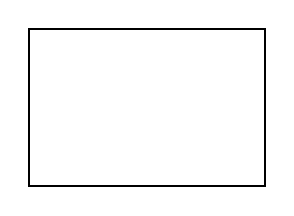
\begin{tikzpicture}
          \node [draw, thick, shape=rectangle, minimum width=3cm, minimum height=2cm, anchor=center] at (0,0) {};
    \end{tikzpicture}
\end{center}
\item The real space lattice has primitive lattice vectors $\mathbf{R_1}=a(1,0)^T$ and $\mathbf{R_2}=b(0,1)^T$. The unit cell is a rectangle of sides $a$ and $b$.
\item As $|t_1|>|t_2|$, there will be more energy contours in the $k_x$ direction than $k_y$ direction. For the contour plot, set $t_1=-1$ and $t_2=-\frac{1}{2}$. We see that
\begin{itemize}
    \item minima: $(k_x,k_y)=\boldsymbol{0}$ at the origin, with effective masses $m_x^*=-\frac{\hbar^2}{2t_1a^2}$ and $m_y^*=-\frac{\hbar^2}{2t_2b^2}$
    \item maxima: $(k_x,k_y)=(\pm\pi,\pm\pi/2)$ at the 4 corners, with effective masses $m_x^*=\frac{\hbar^2}{2t_1a^2}$ and $m_y^*=\frac{\hbar^2}{2t_2b^2}$
    \item saddle points: two pairs at the centre of the BZ edges, $(k_x,k_y)=(\pm\pi,0)$ and $(k_x,k_y)=(0,\pm\pi/2)$, with effective masses $m_x^*=\frac{\hbar^2}{2t_1a^2}$, $m_y^*=-\frac{\hbar^2}{2t_2b^2}$ and $m_x^*=-\frac{\hbar^2}{2t_1a^2}$ and $m_y^*=\frac{\hbar^2}{2t_2b^2}$. The saddle points in the $k_y$ direction are half as high as those in the $k_x$ direction, and have opposite signs of $m^*$ in different directions.
\end{itemize}
where the effective masses are
$$m_i^*=\hbar^2\bigg(\frac{\partial^2E}{\partial k_i^2}\bigg)^{-1}\implies m_x^*=-\frac{\hbar^2}{2t_1a^2}\frac{1}{\cos(ak_x)},\quad m_y^*=-\frac{\hbar^2}{2t_2b^2}\frac{1}{\cos(bk_y)}$$
\item If the energy lies between the minimum and lowest energy saddle point, the contour is closed (electron orbits):
$$E_{\text{min}}<E<\min(E_{\text{sp}})\implies 2(t_1+t_2)<E<2(t_1-t_2)$$
If the energy lies between the highest energy saddle point and maxima, the contour is closed (hole orbits):
$$\max(E_{\text{sp}})<E<E_{\text{max}}\implies 2(-t_1+t_2)<E<2(-t_1-t_2)$$
If the energy lies between the maximum and minimum of saddle point energies, then the contour is open:
$$\min(E_{\text{sp}})<E<\max(E_{\text{sp}})\implies 2(t_1-t_2)<E<2(-t_1+t_2)$$
assuming $t_1<t_2$.
\item In two-dimensions, the peaks in $g(E)$ correspond to saddle points, while $g(E)$ is flat at low and high energies. Along an energy contour, the density of states exhibit a logarithmic divergence.
$$g(E)=\frac{A}{(2\pi)^2}\int_{\text{contour}}\frac{1}{|\boldsymbol{\nabla_k}E|}d\ell\propto\ln|E-E_s|$$
where $E_s$ is the saddle point energy. 
\begin{figure}[H]
    \centering
    \includegraphics[width=\linewidth]{q5.JPG}
    \caption{(Left): Contour plots for $E(\mathbf{k})$; (Right): Density of states $g(E)$}
\end{figure}
\end{enumerate}
\end{ans}
\newpage
\begin{qns}[Graphite]
A single sheet of graphite has two carbon atoms in the unit cell at positions $\mathbf{d_1} = 0$ and $\mathbf{d_2} = (a/\sqrt{3})(0, 1, 0)$. The translation vectors for the two-dimensional hexagonal lattice are $\mathbf{t_1} = (a/2)(1,\sqrt{3},0)$ and $\mathbf{t_2} = (a/2)(−1,\sqrt{3},0)$.\\[5pt]
The electronic configuration of the carbon atom is 1s$^2$2s$^2$2p$^2$, and ignoring the 1s core states, we need to make a band structure from the s, p$_x$, p$_y$ and p$_z$ orbitals. Because s, p$_x$ and p$_y$ orbitals are even under reflection through the plane, and p$_z$ odd, the two sets do not mix. The first three states hybridise to form $\sigma$−bonds with a large gap between the bonding and anti-bonding orbitals. Within this gap lie the $\pi$-orbitals arising from the hybridised p$_z$. The three bonding $\sigma$ orbitals will accommodate 6 electrons per cell, leaving 2 electrons per unit cell in the $\pi$-bands. This question considers the electronic $\pi$-bands only.
\begin{figure}[H]
    \centering
    \includegraphics[scale=0.65]{Q6.JPG}
\end{figure}
\begin{enumerate}[label=(\alph*)]
    \item Construct Bloch states that consist of a linear mixture of the two p$_z$ orbitals in the unit cell, and show how this gives rise to the secular equation to determine the eigenstate energies
    \begin{equation}
        \begin{vmatrix}E_p-E&tF(\mathbf{k})\\tF^*(\mathbf{k})&E_p-E\\\end{vmatrix}=0
    \end{equation}
    where $t$ is the two center hopping matrix element between neighbouring p$_z$ orbitals, and
    \begin{equation}
        F(\mathbf{k})=1+2\cos\frac{k_xa}{2}\exp(-i\sqrt{3}k_ya/2)
    \end{equation}
    \item Show that the reciprocal lattice is also a hexagonal lattice, at an angle of $\pi/6$ to the real-space lattice. Show that the first Brillouin zone is a hexagon centred at the point $\Gamma = (000)$, whose corners are at the points P $= (2\pi/a)(2/3, 0, 0)$.
    \item Determine a formula for the dispersion curves for the two eigenstates, and plot them in the directions $\Gamma$P, and $\Gamma$Q. (Here Q = $(2\pi/a)(1/2, 1/2\sqrt{3},0)$ is at the middle of a zone face.
    \item Where will the $\pi$-bands lie in energy relative to the sp$^2$ $\sigma$- orbitals? Is a single layer of graphite a metal or an insulator?
    \item Carbon nanotubes are formed by curling a graphite sheet into a tube, connecting the atoms with periodic boundary conditions. There are many ways to do this, and the different nanotubes can be indexed by the vector $m\mathbf{t_1} + n\mathbf{t_2}$ that identifies which atoms are connected periodically. Assuming the band-structure is unchanged, show that the allowed k-states now lie on a set of lines whose direction is parallel to the tube. Discuss the situations under which the resulting tube will be semiconducting or metallic.
\end{enumerate}
\end{qns}
\newpage
\begin{ans}\leavevmode
\begin{enumerate}[label=(\alph*)]
\item Let $|p_{z,1}\rangle:=|\alpha\rangle$ and $|p_{z,2}\rangle:=|\beta\rangle$. We want to find a suitable linear combination for the $\pi$ orbitals, i.e. $|\psi\rangle=c_1|\alpha\rangle+c_2|\beta\rangle$ for some $c_1$ and $c_2$. To satisfy Bloch's theorem, we need a tight-binding ansatz of the form
$$|\psi_k\rangle=\sum_{m}e^{i\mathbf{k}\cdot\mathbf{r_m}}(c_1|\alpha\rangle+c_2|\beta\rangle),\quad H|\psi_k\rangle=E_k|\psi_k\rangle$$
Project the Schr\"{o}dinger's equation onto $|\alpha\rangle$ and $|\beta\rangle$ respectively:
$$(E_p-E_k)c_1+t(1+e^{-i\mathbf{t_2}\cdot\mathbf{k}}+e^{-i\mathbf{t_1}\cdot\mathbf{k}})c_2=0$$
$$(E_p-E_k)c_2+t^*(1+e^{i\mathbf{t_2}\cdot\mathbf{k}}+e^{i\mathbf{t_1}\cdot\mathbf{k}})c_1=0$$
where $E_p=\langle\alpha|H|\alpha\rangle=\langle\beta|H|\beta\rangle$, and $\langle\alpha|H|\beta\rangle=t(1+e^{-i\mathbf{t_2}\cdot\mathbf{k}}+e^{-i\mathbf{t_1}\cdot\mathbf{k}})$. We identify this as
$$F(\mathbf{k})=1+e^{-i\mathbf{t_2}\cdot\mathbf{k}}+e^{-i\mathbf{t_1}\cdot\mathbf{k}}=1+e^{iak_x/2}e^{-i\sqrt{3}ak_y/2}+e^{-iak_x/2}e^{-i\sqrt{3}ak_y/2}=1+e^{-i\sqrt{3}ak_y/2}2\cos0.5k_xa$$
\item The reciprocal lattice satisfy:
$$\mathbf{\tilde{t}_1}\cdot\mathbf{\tilde{t}_2}=0\implies\mathbf{\tilde{t}_1}\propto\begin{pmatrix}1\\1/\sqrt{3}\\0\\\end{pmatrix},\quad\mathbf{\tilde{t}_1}\cdot\mathbf{t_1}=2\pi\implies\mathbf{\tilde{t}_1}=\frac{2\pi}{a}\begin{pmatrix}1\\1/\sqrt{3}\\0\\\end{pmatrix}$$
Similarly, $\mathbf{\tilde{t}_2}=\frac{2\pi}{a}(-1,1/\sqrt{3},0)^T$. Since $|\mathbf{\tilde{t}_1}|=4\pi/\sqrt{3}a$ and $|\mathbf{t_1}|=a$, we have
$$2\pi=\frac{4\pi}{\sqrt{3}}\cos\theta\implies\theta=\frac{\pi}{6}$$
Real space lattice and reciprocal space lattice related by $\pi/6$.
\begin{center}
\begin{tikzpicture}
\draw[pattern={hexa with circles[size=10pt,line width=.8pt,angle=90]},
pattern color=blue] (0,0) rectangle ++(2,2); 
\draw[pattern={hexa with circles[size=10pt,line width=.8pt,angle=0]},
pattern color=red] (3,0) rectangle ++(2,2); 
\end{tikzpicture}
\end{center}
The perpendicular bisector connects corners of the hexagon. Projecting half of the length along $\mathbf{t_1}$, we have
$$\frac{1}{2}\frac{2\pi}{a}\sqrt{\frac{4}{3}}\frac{1}{\cos(\pi/6)}=\frac{2\pi}{a}\frac{2}{3}$$
Rotating the coordinates such that one of the corner is on the x-axis. Let this corner be P, then it has coordinates $(2\pi/a)(2/3,0,0)$. 
\item The dispersion relation satisfy
$$(E-E_p)=\pm t|F|$$
where $|F|$ depends on $\mathbf{k}$. For P, $\mathbf{k}=\frac{2\pi}{a}(2/3,0,0)k$,
$$|F|=|1+2\cos\frac{2\pi}{a}\frac{2}{3}\frac{a}{2}k|=|1+2\cos\frac{2\pi}{3}k|$$
and for Q, $\mathbf{k}=\frac{2\pi}{a}(1/2,1/2\sqrt{3},0)k$,
\begin{align}
|F|&=|1+2e^{-i(\sqrt{3}a/2)(2\pi/a)(k/2\sqrt{3})}\cos\frac{\pi}{a}\frac{a}{2}k|\nonumber\\&=\sqrt{(1+2e^{-i\pi k/2}\cos0.5\pi k)(1+2e^{i\pi k/2}\cos0.5\pi k)}\nonumber\\&=\sqrt{1+8\cos^20.5\pi k}\nonumber
\end{align}
\begin{center}
\begin{tikzpicture}
      \draw[->] (-3,0) -- (3,0) node[right] {$k$};
      \draw[->] (0,-3.5) -- (0,3.5) node[left] {$E(k)-E_p$};
      \draw[domain=0:2.1,smooth,variable=\x,red] plot ({\x},{1+2*cos(deg(\x))});
      \draw[domain=-1.57:0,smooth,variable=\x,blue] plot ({\x},{sqrt(1+8*(cos(deg(\x)))^2)});
      \draw[domain=0:2.1,smooth,variable=\x,red] plot ({\x},{-1-2*cos(deg(\x))});
      \draw[domain=-1.57:0,smooth,variable=\x,blue] plot ({\x},{-sqrt(1+8*(cos(deg(\x)))^2)});
      \draw (2.1,0) node[below]{P};
      \draw (0,0) node[below]{$\Gamma$};
      \draw (-1.57,0) node[below]{Q};
\end{tikzpicture}
\end{center}
\item The hybridized sp$^2$ atomic orbitals have a large charge density in the plane of the sheet. The p$_z$ atomic orbitals have a node in the plane of the sheet. It is expected the sp$^2$ orbitals will have a greater overlap between neighbouring atoms than the p$_z$ orbitals. So the energy gap between the sp$^2$ bonding and antibonding orbitals will be greater than the energy gap between the p$_z$ bonding and antibonding orbitals. Hence, we expect the $\pi$ bonding and anti-bonding bands (from p$_z$ orbitals) to lie between the bonding and antibonding bands from the sp$^3$ orbitals. There is one $\pi$-bonding orbital per atom, which are filled with electrons. The $\pi$-antibonding orbitals are empty, the bonding and antibonding states have equal energies at the corners of the Brillouin Zones (P points) so it is possible for a small number of electrons to be excited from filled states to vacant states with a very small energy, and hence graphite has some metallic character. It is actually a semimetal.
\item The lattice vector $m\mathbf{t_1}+n\mathbf{t_2}$ curls around the circumference of the tube in a plane perpendicular to the tube axis. The $\pi$ electron wavefunctions must satisfy the periodic boundary conditions $\psi(\mathbf{r}+m\mathbf{t_1}+n\mathbf{t_2})=\psi(\mathbf{r})$. Bloch's theorem implies $\psi_{\mathbf{k}}(\mathbf{r})=e^{i\mathbf{k}\cdot\mathbf{R}}U(\mathbf{r})$, where $U(\mathbf{r})=U(\mathbf{r}+m\mathbf{t_1}+n\mathbf{t_2})$ with $\mathbf{R}=m\mathbf{t_1}+n\mathbf{t_2}$. 
$$\psi_\mathbf{k}(\mathbf{r}+m\mathbf{t_1}+n\mathbf{t_2})=e^{i\mathbf{k}\cdot(m\mathbf{t_1}+n\mathbf{t_2})}\psi_\mathbf{k}(\mathbf{r})\implies \mathbf{k}\cdot(m\mathbf{t_1}+n\mathbf{t_2})=2\pi N$$
where $N\in\mathbb{Z}$. Define the angle between $\mathbf{k}$ and $m\mathbf{t_1}+n\mathbf{t_2}$ to be $\theta$, then
$$|\mathbf{k}|\cos\theta=\frac{2N\pi}{|m\mathbf{t_1}+n\mathbf{t_2}|}$$ 
i.e. the allowed values of $\mathbf{k}$ lie on lines parallel to the tube axis is constant. The only points in the Brillouin Zone for which the filled and unfilled bands overlap (giving metallic behaviour) are points like P in the zone corners, with wavevectors $\mathbf{k}=\pm\frac{4\pi}{3a}(1,0,0)$, $\pm\frac{4\pi}{3a}(\frac{1}{2},\frac{\sqrt{3}}{2},0)$, $\pm\frac{4\pi}{3a}(-\frac{1}{2},\frac{\sqrt{3}}{2},0)$. For the graphite to be metallic, we obtain an equivalent condition $\forall\mathbf{k}$ values given above.
$$\mathbf{k}\cdot(m\mathbf{t_1}+n\mathbf{t_2})=2N\pi,~N\in\mathbb{Z}\implies\frac{1}{2}(m-n)\in\mathbb{Z}$$
If the condition is obeyed, the nanotube is metallic. If not, there will be an energy gap between the filled and empty states, and the nanotube will be a semiconductor.
\end{enumerate}
\end{ans}
\newpage
\begin{qns}[Band structure of d-band metals]
In many transition metals a narrow d-band lies within a broad energy band originating from s−orbitals. This question discusses the band structure using a simple one-dimensional model constructed from a tight-binding Hamiltonian with one s-orbital $\phi_s(r)$ and one dorbital $\phi_d(r)$ per atom; the atoms are arranged in a linear chain of lattice constant $a$.
\begin{enumerate}[label=(\alph*)]
    \item Write down two Bloch states $\phi_s(k)$ and $\phi_d(k)$ formed from the atomic s- and d- states respectively. The eigenstates must be linear combinations of these.
    \item  Hence show that the one-particle bandstructure E(k) can be found from the determinantal equation
    $$\begin{vmatrix}E_s-2t_{ss}\cos(ka)-E(k)&-2t_{sd}\cos(ka)\\-2t_{sd}\cos(ka)&E_d-2t_{dd}\cos(ka)-E_k\\\end{vmatrix}=0$$
    Identify and explain the parameters appearing in the determinantal equation, and discuss the approximations made that lead to this form.
    \item Discuss why you would expect that $t_{ss} > |t_{sd}| > t_{dd}$.
    \item Plot the dispersion of the two bands when $|E_d − E_s|<< 2|t_{ss}|$, and $t_{sd}$ and $t_{dd}$ are neglected.
    \item How is the dispersion modified from (d) by the inclusion of small values of $t_{sd}$ and $t_{dd}$?
    \item Discuss the relevance of this model to the electronic bandstructure of Cu metal.
\end{enumerate}
\end{qns}
\begin{ans}\leavevmode
\begin{enumerate}[label=(\alph*)]
\item The $s$ and $d$ orbitals for the $m$th atom (with position $x_m=ma$) are
$$\psi_s(x-ma),\quad\psi_d(x-ma)$$
assume they form an orthonormal basis. The tightbinding ansatz give:
$$\phi_k(x)=\frac{1}{\sqrt{N}}\sum_me^{ikma}(c^s_k\psi_s(x-ma)+c^d_k\psi_d(x-ma))$$
\item Plug the eigenstate into the Schr\"{o}dinger's equation:
$$\sum_me^{ikma}\bigg[c_k^s\hat{H}|\psi_s(x-ma)\rangle+c_k^d\hat{H}|\psi_d(x-ma)\rangle\bigg]=\sum_mE_ke^{ikam}\bigg(c^k_s|\psi_s(x-ma)\rangle+c_d^k|\psi_d(x-ma)\rangle\bigg)$$
Project onto $|\psi_s(x-na)\rangle$:
$$e^{ikan}E_kc_{sk}=\sum_me^{ikam}c_{sk}\langle\psi_s(x-na)|\hat{H}|\psi_s(x-ma)\rangle+e^{ikam}c_{dk}\langle\psi_s(x-na)|\hat{H}|\psi_d(x-ma)\rangle$$
We define the overlap $\langle\psi_s(x-na)|\hat{H}|\psi_s(x-ma)\rangle$ to be 
\begin{itemize}
    \item $E_s$ if $n=m$, i.e. the expectation energy of the electron in a pure s-orbital state in the lattice Hamiltonian;
    \item $-t_{ss}$ if $n=m\pm1$, i.e. the hopping matrix element between s-orbitals on adjacent atoms. This is a measure of energy shift due to s-orbital overlap between $n$ orbitals;
    \item zero otherwise
\end{itemize}
The overlap $\langle\psi_s(x-na)|\hat{H}|\psi_d(x-ma)\rangle$ is $t_{sd}$ if $n=m\pm1$, i.e. hopping between s and d-orbital on adjacent atoms. The sign depends on the symmetry of the orbitals. We thus obtain
\begin{align}
&e^{ikam}c_{sk}E_s-e^{ikan}c_{sk}t_{ss}(e^{ika}+e^{-ika})-c_{dk}t_{sd}e^{ikan}(e^{ika}+e^{-ika})=e^{ikam}E_kc_{sk}\nonumber\\
&\implies(E_s-2t_{ss}\cos ka-E_k)c_{sk}-2t_{sd}c_{dk}\cos ka =0\nonumber
\end{align}
Similarly, project onto $|\psi_d(x-na)\rangle$:
$$e^{ikan}E_kc_{dk}=\sum_me^{ikam}c_{dk}\langle\psi_d(x-na)|\hat{H}|\psi_d(x-ma)\rangle+e^{ikam}c_{sk}\langle\psi_d(x-na)|\hat{H}|\psi_s(x-ma)\rangle$$
We define the overlap $\langle\psi_d(x-na)|\hat{H}|\psi_d(x-ma)\rangle$ to be 
\begin{itemize}
    \item $E_d$ if $n=m$, i.e. the expectation energy of the electron in a pure d-orbital state in the lattice Hamiltonian;
    \item $-t_{dd}$ if $n=m\pm1$, i.e. the hopping matrix element between d-orbitals on adjacent atoms. The overlap of two in-phase d-orbital will lower the energy of the pair of atoms;
    \item zero otherwise
\end{itemize}
We thus obtain
\begin{align}
&e^{ikam}c_{dk}E_d-e^{ikan}c_{dk}t_{dd}(e^{ika}+e^{-ika})-c_{sk}t_{sd}e^{ikan}(e^{ika}+e^{-ika})=e^{ikam}E_kc_{dk}\nonumber\\
&\implies(E_d-2t_{dd}\cos ka-E_k)c_{dk}-2t_{sd}c_{sk}\cos ka =0\nonumber
\end{align}
Matriculate both equations:
$$\begin{pmatrix}E_s-2t_{ss}\cos(ka)-E(k)&-2t_{sd}\cos(ka)\\-2t_{sd}\cos(ka)&E_d-2t_{dd}\cos(ka)-E_k\\\end{pmatrix}\begin{pmatrix}c_{sk}\\c_{dk}\\\end{pmatrix}=0$$
Set the determinant to be zero, in order to find non-trivial solutions, which will give
$$(E_s-2t_{ss}\cos(ka)-E(k))(E_d-2t_{dd}\cos(ka)-E(k))-4t_{sd}^2\cos^2ka=0$$
\item In 3d transition metal, the 3d and 4s orbitals overlap to form bands. As seen from the radial distributions, the electron density is concentrated closer to the nucleus for 3d than for 4s. The overlap for s-orbitals on adjacent atoms will be much greater than the overlap between s- and d-orbitals on adjacent atoms. In turn, this overlap will be greater than the overlap between d-orbitals on adjacent atoms. Hence,
$$t_{ss}>|t_{sd}|>|t_{dd}|$$
\item When $|E_d-E_s|<<2|t_{ss}|$ and $t_{sd},t_{dd}\approx 0$, we have
$$0=(E_s-2t_{ss}\cos(ka)-E(k))(E_d-2t_{dd}\cos(ka)-E(k))-4t_{sd}^2\cos^2ka\approx(E_s-2t_{ss}\cos(ka)-E(k))(E_d-E(k))$$
which gives $E(k)=E_d$ or $E(k)=E_s-2t_{ss}\cos ka$. The s-orbitals overlap strongly to form a wide band of energy levels. In this approximation, d orbitals do not interact. There is an isolated d-orbital in each atom, $E_d$ form a very narrow band of $d$-states.
\item When $t_{dd}\neq 0$, we have
\begin{align}
&(E_s-2t_{ss}\cos(ka)-E(k))(E_d-2t_{dd}\cos(ka)-E(k))-4t_{sd}^2\cos^2ka\nonumber\\&\approx(E_s-2t_{ss}\cos(ka)-E(k))(E_d-2t_{dd}\cos(ka)-E(k))\nonumber
\end{align}
which gives $E(k)=E_s-2t_{ss}\cos(ka)$ or $E(k)=E_d-2t_{dd}\cos ka$. The very narrow d-band is now broadened.\\[5pt]
As $t_{sd}$, the overlap between s- and d-orbitals, is increased, the hybridization results in avoided crossings of $s$ and $d$ orbitals. Specifically, we have the solutions
$$E_k=\frac{\tilde{E}_s+\tilde{E}_d}{2}\pm\frac{1}{2}\sqrt{(\tilde{E}_s-\tilde{E}_d)^2+16t^2_{sd}\cos^2ka},\quad\tilde{E}_s=E_s-2t_{ss}\cos ka,\quad\tilde{E}_d=E_d-2t_{dd}\cos ka$$
\item In Cu metal, the 3d and 4s orbitals interact in this way. In its bandstructure, the narrow 3d band is in the middle of the 4s band, with avoided crossings created due to band hybridization. This provides a possible route for optical excitation of electrons from 3d to 4s, and because the energies involved are in the visible spectrum. The reflectivity exhibits an energy dependence, and hence Cu metal appears red.
\end{enumerate}
\end{ans}
\newpage
\section{Problem Sheet 3}
\subsection*{Band structure probes}
\begin{qns}[Quantum oscillations and band structure in Sr$_2$RuO$_4$]
A square lattice of ruthenium, Ru, atoms forms the key structural element of the layered compound Sr$_2$RuO$_4$. Three of the five Ru d-orbitals are degenerate and contribute to the band structure close to the Fermi energy: $|d_{xy}\rangle$, $|d_{xz}\rangle$ and $|d_{yz}\rangle$. The $d_{xy}$ orbitals hybridise with those of neighbours in the $x$- and $y$- direction, the $d_{xz}$ orbitals only hybridise with those of neighbours along the $x$-direction, and the $d_{yz}$ orbitals only hybridise with those of neighbours along the $y$-direction. Hybridisation along the $z$-direction is negligible. Four electrons per Ru are distributed equally across the three bands arising from the hybridisation of these orbitals. 
\begin{figure}[H]
    \centering
    \includegraphics[width=\linewidth]{q3_1.JPG}
    \caption{de Haas van Alphen signal measured with $B\parallel c$ in Sr$_2$RuO$_4$. Upper panel: experimental raw data. Lower panel: Fourier transformed data, showing fundamental frequencies corresponding to three Fermi surface sheets, $\alpha$, $\beta$ and $\gamma$.}
\end{figure}
Hybridisation between the $|d_{xy}\rangle$ orbitals gives rise to the $\gamma$ Fermi surface sheet, which can be approximated as a cylinder pointing along the $c^∗$-direction with a circular crosssection in the $a^∗b^∗$ plane. Use data from Fig. 1 to determine the Fermi wavevector $k_F$ characterising this cylinder and to estimate the lattice constant a of the square Ru lattice.\\[5pt]
Nearest neighbour hybridisation between the $|d_{xz}\rangle$ orbitals gives rise to Fermi surface sheet A, whereas hybridisation between the $|d_{yz}\rangle$ orbitals leads to Fermi surface sheet B. Sketch the three Fermi surface sheets A, B and $\gamma$ and state their characteristic dimensions.\\[5pt]
A higher order mechanism induces a small hybridisation between the $|d_{xz}\rangle$ and $|d_{yz}\rangle$ orbitals, which causes two new Fermi surface sheets, $\alpha$ and $\beta$ to emerge from sheets A and B. Relate the dimensions of these sheets to the corresponding de Haas van Alphen frequencies in Fig. 1. Which of these sheets would you expect to be a hole sheet?
\end{qns}
\newpage
\begin{ans}
4 electrons are distributed equally across 3 bands. Hybridization between $|d_{xy}\rangle$ gives $\gamma$ surface, contributed by on average $\frac{4}{3}$ number of electrons. $\gamma$ is cylindrical with 2D circular cross-section
$$2\pi k_F^2\frac{a^2}{(2\pi)^2}=\frac{4}{3}$$
where 2 is the spin degeneracy factor. The circular cross-section has area
$$A_k=\pi k_F^2=\frac{2}{3}\frac{(2\pi)^2}{a^2}$$
i.e. $\gamma$ takes up $2/3$ of the Brillouin Zone. Fig. 1 gives $\frac{1}{\Delta(1/B)}\sim 18$ kT for $\gamma$. The Onsanger relation gives:
$$A_k=\frac{2\pi e}{\hbar}\frac{1}{\Delta(1/B)}\implies a=\sqrt{\frac{2}{3}(2\pi)^2\frac{\hbar}{e}\Delta(1/B)}=\sqrt{\frac{2}{3}\frac{6.62\times10^{-34}}{1.6\times10^{-19}}\frac{1}{18\times10^3}}=3.92~\angstrom$$
$|d_{xz}\rangle$ and $|d_{yz}\rangle$ hybridize with nearest neighbours along the $x$- and $y$-directions respectively. Using the tight-binding ansatz $|k\rangle=\sum_ne^{i\mathbf{k}\cdot\mathbf{R_n}}|d^n\rangle$, the dispersion relations for Fermi sheets A and B respectively give
$$E_x(k)=\langle d_{xz}|H|k\rangle=E_0+t_x\cos k_xa,\quad E_y(k)=E_0+t_y\cos k_ya$$
A and B are thus plane Fermi sheets with spacing $\frac{2}{3}\frac{2\pi}{a}$.\\[5pt]
Further hybridization between A and B gives sheets $\alpha$ and $\beta$, illustrated in \url{https://bit.ly/3rehbOQ}. The areas enclosed by the sheets are
$$A_\alpha\sim\bigg(\frac{1}{3}\frac{2\pi}{a}\bigg)^2=\frac{1}{9}\frac{3}{2}A_\gamma\propto\frac{1}{9}\frac{3}{2}18\times10^3=3~\text{kT}$$
$$A_\beta\sim\bigg(\frac{2}{3}\frac{2\pi}{a}\bigg)^2=\frac{2}{3}A_\gamma\propto\frac{2}{3}18\times10^3=12~\text{kT}$$
where $\alpha$ is a hole sheet, so it contains the remaining $1/3$ of the Brillouin Zone.
\end{ans}
\begin{qns}[de Haas-van Alphen period of potassium]
Calculate the period ∆(1/B) expected for potassium within the free electron model. What is the area in real space of the extremal orbit, for B = 1 T?
\end{qns}
\begin{ans}
Potassium is a bcc crystal, with 2 atoms per conventional unit cell. The free electron model's Fermi wavevector is $k_F^3=3\pi^2N/V$. The area enclosed by the Fermi surface is
$$A_k=\pi k_F^2=\pi(3\pi^2N/V)^{2/3}=\pi\bigg(3\pi^2\frac{2}{(5.23)^3\angstrom^3}\bigg)^{2/3}=1.74~\angstrom^{-2}$$
The Onsager relation gives the period to be
$$\Delta(1/B)=\frac{2\pi e}{\hbar}\frac{1}{A_k}=\frac{2\pi(1.6\times10^{-19})}{6.626\times10^{-34}/2\pi}\frac{1}{1.74\times10^{20}}=5.48\times10^{-5}~\text{T}^{-1}$$
The real space area is related to $A_k$ via
$$A_r=\frac{\hbar^2}{e^2B^2}A_k=\bigg(\frac{6.626\times10^{-34}/2\pi}{1.6\times10^{-19}}\bigg)^21.74\times10^{20}=7.56\times10^9~\angstrom^2$$
\end{ans}
\newpage
\subsection*{Semiconductors}
\begin{qns}[Band gaps and effective masses]
Using the one-dimensional nearly-free electron result for the energy levels at the Brillouin zone boundary $k = \pi/a$
\begin{equation}
    E^\pm(\mathbf{k})=\frac{1}{2}\frac{\hbar^2}{2m}(k^2+(k-2\pi/a)^2\pm\frac{1}{2}\sqrt{\bigg[\frac{\hbar^2}{2m}(k^2-(k-2\pi/a)^2)\bigg]^2+4|U_0|^2}\label{3_1}
\end{equation}
calculate the effective masses of electrons and hole states in terms of the band gap.\\[5pt]
Is the data in the table below approximately consistent with your result?
\begin{center}
    \begin{tabular}{|c|c|c|}
    \hline
        Crystal  &  $m_e^*$ & $E_{\text{gap}}/eV$ \\
        \hline
        InSb & 0.015 & 0.23\\
        \hline
        InAs & 0.026 & 0.43\\
        \hline
        InP & 0.073 & 1.42\\
        \hline
    \end{tabular}
\end{center}
\end{qns}
\begin{ans}
Write Eqn.~\ref{3_1} near $k=\frac{\pi}{a}+\delta k:=k_0+\delta k$:
\begin{align}
    E_k&=\frac{1}{2}\frac{\hbar^2}{2m}\bigg((k_0+\delta k)^2+(k_0+\delta k-2k_0)^2\bigg)\pm\frac{1}{2}\frac{\hbar^2}{2m}\bigg[\bigg[(k_0+\delta k)^2-(k_0+\delta k-2k_0)^2\bigg]^2+\frac{4U_0^2}{(\hbar^2/2m)^2}\bigg]^{1/2}\nonumber\\&\approx\frac{\hbar^2}{2m}\bigg[k_0^2+\delta k^2\pm\frac{U_0}{\hbar^2/2m}\bigg(1+\bigg(\frac{\hbar^2}{2m}\bigg)^2+\frac{4k_0^2\delta k^2}{2U_0^2}\bigg)\bigg]\nonumber\\&=E_0\pm\bigg(U_0+\frac{2E}{U_0}\frac{\hbar^2}{2m}\delta k^2\bigg)+\frac{\hbar^2}{2m}\delta k^2\nonumber
\end{align}
The effective mass is $m^*=\hbar^2/(\partial^2E/\partial\delta k^2)$:
$$\frac{1}{m^*}=\frac{1}{m}\pm\frac{1}{m}\frac{2E}{U_0}\sim\frac{2E}{mU_0}=\frac{4E_0}{mE_g}\implies\frac{m^*}{m}\approx\frac{E_g}{4E_0}$$
where $U_0<<E$ and $E_g=2U_0$. Take the ratio of $m^*/E_{\text{gap}}$, they are about 0.05 to 0.065, approximately constant, as suggested by the relation we have obtained.
\end{ans}
\begin{qns}[Hole statistics]
Show that $f_h(\epsilon)=1-f_e(\epsilon)$, where
$$f_e(\epsilon)=\frac{1}{e^{\beta(\epsilon-\mu)}+1}$$
is the Fermi distribution function for electrons and
$f_h(\epsilon)=1-f_e(\epsilon)$, where
$$f_h(\epsilon)=\frac{1}{e^{\beta(\mu-\epsilon)}+1}$$
describes the distribution function for holes.
\end{qns}
\begin{ans}
$$1-f_e(\epsilon)=\frac{1+e^{\beta(\epsilon-\mu)}-1}{e^{\beta(\epsilon-\mu)}+1}=\frac{1}{e^{\beta(\mu-\epsilon)}+1}=f_h(\epsilon)$$
\begin{center}
    \begin{tikzpicture}
    \draw [->] (0, 0) -- (5, 0) node [right] {$\epsilon$};
    \draw [->] (0, 0) -- (0, 3) node [above] {$f_e(\epsilon)$};

    \draw [thick] (0, 2) -- (1.8, 2) .. controls (2, 2) and (2, 0) .. (2.2, 0) -- (4.9, 0);

    \node [below] at (2, 0) {$\mu$};
    \draw [decoration={markings, mark=at position 0 with {\arrowreversed{latex'}}, mark=at position 1 with {\arrow{latex'}}}, postaction={decorate}] (1.8, 2.2) -- (2.2, 2.2) node [pos=0.5, above] {$k_BT$};
  \end{tikzpicture}
  \begin{tikzpicture}
    \draw [->] (0, 0) -- (5, 0) node [right] {$\epsilon$};
    \draw [->] (0, 0) -- (0, 3) node [above] {$f_h(\epsilon)$};

    \draw [thick] (4.9 , 2) -- (2.2, 2) .. controls (2, 2) and (2, 0) .. (1.8, 0) -- (0,0);

    \node [below] at (2, 0) {$\mu$};
    \draw [decoration={markings, mark=at position 0 with {\arrowreversed{latex'}}, mark=at position 1 with {\arrow{latex'}}}, postaction={decorate}] (1.8, 2.2) -- (2.2, 2.2) node [pos=0.5, above] {$k_BT$};
  \end{tikzpicture}
\end{center}
The density of holes increases with energy $\epsilon$. The distribution function is such that $f_h(\epsilon)+f_e(\epsilon)=1$, i.e. conserved.
\end{ans}
\newpage
\begin{qns}[Ge]
Give a brief explanation of the concepts of drift velocity, electron mobility, and effective mass, as used in solid state physics.\\[5pt]
A sample of Ge is doped so that the concentration of pentavalent donor impurities, $N_d$ is $3\times10^{22}$ m$^{−3}$, and that of trivalent acceptors, $N_a$, is $10^{22}$ m$^{−3}$. Estimate the concentration of electrons in the conduction band and holes in the valence band at 300 K.\\[5pt]
[The intrinsic carrier density of Ge at 300K is $2.4\times10^{19}$ m$^{-3}$.]\\[5pt]
Sketch a graph of the conductivity as a function of temperature you would expect to measure for this sample of Ge.
\end{qns}
\begin{ans}
The drift velocity $\mathbf{v}$ is the group velocity averaged over all occupied states.
$$\mathbf{v}=\frac{1}{\hbar}\boldsymbol{\nabla_k}E(\mathbf{k})$$
For $\mathbf{B}=0$, in the steady state $\frac{\partial}{\partial t}=0$, we have $\mathbf{v}=-\frac{e\tau}{m}\mathbf{E}$. By defining the electron mobility as
$$\mu=\frac{|\mathbf{v}|}{|\mathbf{E}|}=\frac{e\tau}{m}$$
The effective mass is defined as $m^*=\hbar^2/(\partial^2E(\mathbf{k})/\partial k^2)^{-1}$, and have the usual classical interpretation in the semi-classical model, i.e. $\hbar k=m^*v_g$. $m^*$ is direction-dependent for an anisotropic band strucutre, since it describes its curvature in a particular direction.\\[5pt]
Since $N_d,N_a>>n_i$ in doped Ge, we are in the extrinsic regime. The concentration of electrons and holes satisfy the law of mass action via:
$$np=n_i^2,\quad n=N_d-N_a=2\times10^{22}\text{m}^{-3}\implies p=n_i^2/n=\frac{(2.4\times10^{19})^2}{2\times10^{22}}=2.9\times10^{16}\text{m}^{-3}$$
\begin{center}
\begin{tikzpicture}
      \draw[->] (0,0) -- (3,0) node[right] {$T$};
      \draw[->] (0,0) -- (0,3) node[left] {$\sigma$};
      \draw[domain=0:2,smooth,variable=\x,black] plot ({\x},{\x*\x*\x-2*\x*\x+\x+1});
      \draw (1.1,0) node[below]{300K};
      \draw (0,0) node[below]{0};
\end{tikzpicture}
\end{center}
where the intrinsic carriers dominate at high temperatures, but at temperatures lower than room temperature, it is in the extrinsic regime.
\end{ans}
\begin{qns}[Impurity bands]
InSb has a dielectric constant $\epsilon=18$ and an effective mass for electrons $m^∗ = 0.015m$. Calculate the ionisation energy of a hydrogenic donor orbit.\\[5pt]
At what density of donors do you expect to see the effects of overlaps between the orbits of adjacent impurities?\\[5pt]
\textit{At low densities, donor levels are isolated, and if the temperature is so low that the probability of ionisation is very small, the system will be an insulator. But at higher density, the donor levels overlap to form an impurity band that can support metallic conduction.}
\end{qns}
\begin{ans}
The ionization energy and radius of the donor orbit are respectively
$$E_0=\frac{13.6}{\epsilon^2}\frac{m^*}{m_0}=\frac{13.6}{18^2}0.015=0.63\text{meV},\quad r_0=a_0\epsilon\frac{m}{m^*}=\frac{18*5.3\times10^{-11}}{0.015}=636\angstrom$$
The impurity band forms when the distance between donors becomes comparable to $a_0$. This happens at donor density $\sim 4\times10^{21}$ m$^{-3}$.
\end{ans}
\newpage
\section{Problem Sheet 4}
\subsection*{Semiconductor devices}
\begin{qns}[Depletion layer]
\textit{A full treatment of this problem requires the solution of the Poisson equation to determine the electric field distribution $V(x)$ combined with the thermal carrier statistics to determine the occupancy of the states. At low temperature, when the boundary of the depletion regime may be assumed to be sharp, it is more straightforward.}\\[5pt]
A metal-semiconductor contact is made between a perfect conductor and a uniformly doped n-type semiconductor with a donor density $N_d$. Assume that the temperature is low enough that the donor levels are completely filled or completely empty. By solving Poisson's equation, show that in the depletion region $0 < x < x_b$ the potential
$$\phi=\phi_b-\frac{N_de}{2\varepsilon\varepsilon_0}(x_b-x)^2$$
Estimate the depletion width for a semiconductor with $\varepsilon=12$, $e\phi_b=0.5$ eV, and $N_d=10^{22}$ m$^{-3}$.
\end{qns}
\begin{ans}
Let the regions $x<0$ and $x>0$ be the metal and semiconductor respectively. Define the depletion region to occur at $0<x<x_b$. Here, the charge density is $eN_d$ (positive ionized donors) while the region $x>x_b$ is neutral. The electric field in the metal ($x<0$) and the neutral portion of the semiconductor ($x>x_b$) must be zero. Hence, $\phi$ is constant in both regions. $\mathbf{E}$ can be discontinuous at the interface between the metal and semiconductor where there is a change in relative permittivity, but must be continuous between the depletion region and the neutral semiconductor at $x=x_b$. $\phi$ is also continuous at the $x=x_b$ interface.\\[5pt]
By Poisson's equation (in one-dimension), 
$$\frac{\partial^2\phi}{\partial x^2}=-\frac{\rho}{\varepsilon\varepsilon_0}\implies\phi=-\frac{x^2\rho}{2\varepsilon\varepsilon_0}+c_1x+c_2,\quad 0<x<x_b$$
and $\phi=\phi_b$ at $x>x_b$. Invoke the boundary conditions: $\phi$ and $E=-\frac{\partial\phi}{\partial x}$ continuous at $x=x_b$. 
$$\phi=\phi_b-\frac{eN_d}{2\varepsilon\varepsilon_0}(x-x_b)^2$$
Finally, $\phi=0$ for $x\leq 0$, hence $\phi_b=\frac{N_de}{2\varepsilon\varepsilon_0}x_b^2$. This gives
$$x_b=\sqrt{\frac{2\varepsilon\varepsilon_0\phi_b}{eN_d}}=\sqrt{\frac{2(12)(8.85\times10^{-12})(0.5)}{1.6\times10^{-19}(10^{22})}}=257~\text{nm}$$
\end{ans}
\begin{qns}[Quantum well sub-bands]
A 10 nm thick quantum well of GaAs is surrounded by bulk Al$_{0.7}$Ga$_{0.3}$As. The conduction band offset is 0.26 eV, and the effective mass of electrons in GaAs is 0.066 $m_e$.
\begin{enumerate}[label=(\alph*)]
\item Estimate the energies of the (bottom of the) sub-bands $E_n(\mathbf{k} = 0)$, assuming the walls of the potential are infinitely high.
\item What is the maximum areal density of electrons that can be occupied in the lowest sub-band before the second sub-band starts to be filled?
\item How many sub-bands do you estimate exist for the actual situation -  a well of finite potential depth?
\end{enumerate}
\textit{Note the word estimate in (c). Nevertheless, the 1D finite potential well is not a difficult problem to solve, though the actual solution of eigenstate energies needs to be done graphically.}\\[5pt]
For a potential of depth $V_0$ and width $L$, show that the number of bound states
$$1+\text{Int}\bigg[(2m^*V_0L^2/\pi^2\hbar^2)^{1/2}\bigg]$$
\end{qns}
\newpage
\begin{ans}\leavevmode
\begin{enumerate}[label=(\alph*)]
\item If electrons are confined to a $L=10$ nm quantum well, then they will be free to move in 2-dimensions $(x,y)$, but confinement in the third dimension $(z)$ will cause a series of quantized energy levels. This is an infinite well problem, with quantized wavevectors $k_n=n\pi/L$. The energies are
$$E_n=\frac{\hbar^2k_n^2}{2m^*}=\frac{(6.626\times10^{-34}/(2\pi))^2n^2\pi^2}{2(0.066)(9.11\times10^{-31})(10\times10^{-9})^2}=57n^2~\text{meV}$$
where $m^*=0.066m_e$.
\item Assume the system is a square of side $D$ with quantum well dimension $L$ in the $z$-direction, and $D>>L$. The periodic boundary conditions are $k_x=\frac{n_x\pi}{D}$, $k_y=\frac{n_y\pi}{D}$ and $k_z=\frac{n_z\pi}{L}$. The dispersion relation is
$$E=\frac{\hbar^2}{2m^*}(k_x^2+k_y^2+k_z^2)=\frac{\hbar^2\pi^2}{2m^*}\bigg(\frac{n_x^2}{D^2}+\frac{n_y^2}{D^2}+\frac{n_z^2}{L^2}\bigg)=\frac{\hbar^2}{2m^*}(k_x^2+k_y^2)+\frac{\hbar^2\pi^2}{2m^*}\frac{n_z^2}{L^2}$$
Assuming $E_{xy}=\frac{\hbar^2k^2}{2m^*}$, and since the levels are very closely spaced, they are almost continuous. The number of states is
$$g(E_{xy})dE_{xy}=\frac{2(2\pi k)dk}{(2\pi)^2/D^2}=\frac{2(2\pi k)}{(2\pi)^2/D^2}\frac{2m^*}{2\hbar^2k}dE_{xy}\implies g(E_{xy})=\frac{D^2m^*}{\pi\hbar^2}$$
i.e. constant density of states. The energy of subbands $E_n=\frac{\hbar^2n^2\pi^2}{2m^*L^2}$. The difference in energy between the lowest sub-band and the second subband is $\Delta E_n=\frac{3\hbar^2\pi^2}{2m^*L^2}$. The number of states per unit area between these two subbands is
$$n=\frac{N}{D^2}=\frac{g(E_{xy})\Delta E_n}{D^2}=\frac{D^2m^2}{\pi\hbar^2}\frac{3\hbar^2\pi^2}{2m^*L^2}\frac{1}{D^2}=\frac{3\pi}{2(10\times10^{-9})^2}=4.71\times10^{16}\text{m}^{-2}$$
\item The energies are $E_1=57(1)^2$ meV and $E_2=57(2)^2$ meV. The band offset is 260 meV. This is the depth of finite well. If we assume energy levels for the finite square well are at the infinite well values, then both subbands 1 and 2 can be occupied.
\end{enumerate}
The wavefunction solutions with the finite well are similar to the infinite well with exponential tails propagating into barriers. 
\begin{equation}
  \psi(z) =
    \begin{cases}
      Ae^{\alpha z} & z<-L/2\\
      Be^{ik_zz}+Ce^{-ik_zz} & |z|<L/2\\
      De^{-\alpha z} & z>L/2
    \end{cases}       
\end{equation}
with energy $E_z=\frac{\hbar^2k_z^2}{2m^*}=V_0-\frac{\hbar^2\alpha^2}{2m^*}$. The Hamiltonian is invariant under reflection about $z=0$ $\implies\psi(z)=\pm\psi(-z)\implies A=\pm D$, $B=\pm C$. The boundary conditions are $\psi(z)$, $\psi'(z)$ continuous at $z=\pm L/2$. The even and odd solutions respectively are
$$B=C\implies\alpha\frac{L}{2}=k_z\frac{L}{2}\tan(k_zL/2)$$
$$B=-C\implies\alpha\frac{L}{2}=k_z\frac{L}{2}\cot(k_zL/2)$$
By finding the intersection of these curves with circles $\gamma^2=\frac{L}{2}(\alpha^2+k_z^2)=\frac{m^*V_0L^2}{2\hbar^2}$, we can find the number of allowed $(\alpha,k_z)$ solutions, which is
$$n=\text{Int}\bigg[\sqrt{\frac{m^*V_0L^2}{2\hbar^2}}\frac{1}{\pi/2}\bigg]+1$$
where each solution occurs near the asymptotes near $m\pi/2$, $m\in\mathbb{Z}$.
\end{ans}
\newpage
\begin{qns}[Brief notes 1]
Write brief notes about
\begin{itemize}
    \item p-n junctions and the p-n junction diode I-V characteristic.
    \item Light emitting diodes and solar cells.
    \item Field effect transistors.
\end{itemize}
\end{qns}
\begin{ans}\leavevmode
\begin{itemize}
\item The p-n junction diode is formed by connecting a p-type and a n-type semiconductor together. When they are in contact, current flow equalizes the chemical potential across both materials, causing electrons to diffuse from the n-side to the p-side, and holes to diffuse from the p-side to the n-side. This creates a depletion layer where virtually no charge carriers are present with a positively charged n-side (due to electrons leaving the dopant cores) and a negatively charged p-side (due to holes leaving the dopant core).\\[5pt]
There is a balance between the recombination/diffusion current for carriers to go across the potential barrier and the drift/generation current, due to electron-hole pair formation as a result of thermal excitations, when there is no applied field.\\[5pt]
In reverse bias, the barrier height is raised, and the diffusion current is negligible such that a small current is present due to the dominant drift current. In forward bias, the barrier height is reduced and the diffusion current dominates significant. This behaviour is captured by the diode equation
$$I=I_{\text{sat}}(e^{eV/k_BT}-1)$$
Under strong reverse bias, the Zener breakdown or avalanche breakdown can occur such that there can be a finite large current in reverse bias.
\item Light emitting diodes are p-n junctions optimized for the production of photons during carrier recombination. In forward bias, the electrons and holes are injected towards the interface, where they recombine and emit a photon with an energy close to the bandgap (i.e. the electrons undergo transitions from the conduction band to the valence band).\\[5pt]
The working principle of solar cells is the converse of LEDs - when a photon is absorbed, electron-hole pairs are formed, which are accelerated by the in-built electric field in the depletion layer. This generates a drift current that can be harnessed for power. The Shockley-Quisser limit gives the maximum efficiency of solar cells that can be achieved by bandgap tuning, about 33 percent for an $E_{\text{gap}}=1.2$ eV.
\item Field effect transitions are transistors that use electric fields to control the flow of current. They have 3 terminals - the gate, source and drain. The working principle is based on using the voltage applied to the gate to manipulate the charge carrier density in the channel between the source and the drain.\\[5pt]
Junction-based FETs (JFETs) use p-n junctions to control the width of the conducting channel and therefore the current between the source and the drain. By design, JFETs contain free electrons and channel for the conduction, hence they can operate only in depletion mode\\[5pt]
Metal oxide semiconductor FETs (MOSFETs) has a similar working principle but has the advantage that the gate electrode is electrically insulated from the rest of the device, so that there is no current flow from the gate electrodes. Also, MOSFETs can be used in enhancement mode as well as depletion mode.
\end{itemize}
\end{ans}
\newpage
\subsection*{Interacting electron systems}
\begin{qns}[Peierls transition]
Consider a one-dimensional system which is filled up to the first Brillouin zone boundary at $k =\pi/a$, and assume that there is a small gap produced by a single Fourier component of the lattice potential $U = U_{K=2\pi/a}$ (small meaning that $U/E^0_{K/2}<<1$). Consider momenta close to the zone boundary, and show that a good approximation for the energy dispersion of the bands is
$$E=E_0\bigg(1\pm\sqrt{\frac{U^2}{E_0^2}+4\kappa^2}\bigg)$$
where $E_0=E^0_{K/2}$ and $k=(\pi/a)(1+\kappa)$, with $\kappa<<1$.\\[5pt]
Show that the change in electronic energy
$$E_{\text{elec}}=\frac{1}{N}\sum_{k \text{ occupied}}[E(k;U_K)-E(k;U_K=0)]$$
can be written approximately as
$$E_{\text{elec}}=|U|\int_0^1\bigg[\frac{x}{\alpha}-\bigg(1+\frac{x^2}{\alpha^2}\bigg)^{1/2}\bigg]\propto\frac{\hbar^2\pi^2}{ma^2}\alpha^2\log\alpha$$
in the limit that the parameter $\alpha=\frac{ma^2}{\hbar^2\pi^2}|U|$ is much smaller than unity (i.e. the gap is small compared to the bandwidth.)
\end{qns}
\begin{ans}
The nearly free electrons approximation is valid close to the zone boundary at $k\approx \pi/a$ and for a lattice potential $U(x)=2U_K\cos(2\pi x/a)$, where $a$ is the lattice constant. The energies are
$$E_\pm(k)=\frac{\hbar^2}{2m}\frac{1}{2}\bigg(k^2+\bigg(k-\frac{2\pi}{a}\bigg)^2\bigg)\pm\frac{1}{2}\sqrt{\bigg(\frac{\hbar^2}{2m}\bigg)^2\bigg(k^2-\bigg(k-\frac{2\pi}{a}\bigg)^2\bigg)^2+4U_K^2}$$
Let $k=\frac{\pi}{a}(1+\kappa)$, where $|\kappa|<<1$, i.e. $k\approx\pi/a$, then
$$k^2\pm\bigg(k-\frac{2\pi}{a}\bigg)^2=\frac{\pi^2}{a^2}\bigg[(1+\kappa)^2\pm(\kappa-1)^2\bigg]$$
For $\kappa<<1$, this gives
$$E_\pm(\kappa)= E_0\frac{1}{2}\bigg[(1+\kappa)^2+(-1+\kappa)^2\bigg]\pm E_0\sqrt{((1+\kappa)^2-(-1+\kappa)^2)^2+\frac{4U^2}{E_0^2}}\approx E_0\bigg(1\pm 2\sqrt{\kappa^2+\frac{U^2}{4E_0^2}}\bigg)$$
where we neglected $\kappa^2$ outside of the square root. Let $N$ be the number of spatial states, and is large, then the change in electronic energy is
\begin{align}
    \Delta E=\frac{1}{N}\sum_{k~\text{occupied}}\bigg[E_k(U_K)-E_k(U_K=0)\bigg]&=\frac{1}{N}\sum_{n=-N/2}^{N/2}\bigg[E_{k_n}(U_K)-\frac{\hbar^2k_n^2}{2m}\bigg]\nonumber\\&\approx\frac{1}{N}\int_{-N/2}^{N/2}E(k_n,U_K)-\frac{\hbar^2k_n^2}{2m}dn\nonumber\\&=\frac{a}{2\pi}\int_{-\pi/a}^{\pi/a}E(k,U_K)-\frac{\hbar^2k^2}{2m}dk\nonumber\\&\approx\int_{-1}^0\bigg[E_0(1+\kappa^2)-E_0\sqrt{4\kappa^2+\frac{U_K^2}{E_0^2}}-E_0(1+\kappa)^2\bigg]d\kappa\nonumber\\&=\int_0^12xE_0-E_0\sqrt{4x^2+\frac{U_K^2}{E_0^2}}dx\nonumber\\&=\int_0^12x\frac{|U_K|}{2\alpha}-\frac{|U_K|}{2\alpha}\sqrt{4x^2+\frac{4\alpha^2U_K^2}{|U_K|^2}}dx\nonumber\\&=|U_K|\int_0^1\frac{x}{\alpha}-\sqrt{\frac{x^2}{\alpha^2}+1}dx\nonumber
\end{align}
where $k_n=\frac{2\pi n}{Na}\implies dn=\frac{Na}{2\pi}dk$, and we take the $E_-$ solution. Finally, we made the substitutions $x=-\kappa$ and $\alpha=\frac{ma^2}{\hbar^2\pi^2}|U_K|=\frac{|U_K|}{2E_0}$. To evaluate the integral, substitute $x=\alpha\sinh\theta$.
$$\frac{\Delta E}{|U_K|}=\frac{1}{2\alpha}-\int_0^{\sinh^{-1}(1/\alpha)}\alpha\cosh^2\theta d\theta=\frac{1}{2\alpha}-\frac{\alpha}{2}\sinh^{-1}\frac{1}{\alpha}-\frac{1}{2}\sqrt{1+\frac{1}{\alpha^2}}\approx-\frac{\alpha}{2}\ln\frac{2}{\alpha}$$
where for $\alpha<<1$, $\frac{1}{2}\sqrt{1+\frac{1}{\alpha^2}}\approx\frac{1}{2\alpha}$ and $\sinh\alpha\approx\frac{1}{2}e^\alpha$. Since $|U_K|\propto\alpha$, the result follows.
\end{ans}
\begin{qns}[Covalent bonds are singlets]
\textit{How is it that electrons in a covalent bond - e.g. H$_2$ - are almost invariably in singlet states? The two atomic states that make up the wavefunction are not orthogonal, and so the charge density is not independent of the spin-state of the ions. The singlet state will lead to a charge density that is more favourable for strong bonds than the triplet.}
\begin{figure}[H]
    \centering
    \includegraphics[scale=0.75]{Q4_5.JPG}
    \caption{A sketch of the charge density for the wavefunctions in a singlet state (solid line) and
a triplet state(dotted line) for two overlapping gaussian orbitals in (3)}
    \label{fig:1}
\end{figure}
Consider single-particle wavefunctions on two neighbouring identical atoms  A,  B, which may be assumed real. These are to be used as the basis for a two-electron state. Show that the charge density in a singlet (triplet) state made out of the two orbitals is given by
\begin{equation}
    \rho(r)=|\psi_A(r)|^2+|\psi_B(r)|^2\pm 2\langle\psi_A|\psi_B\rangle\psi_A(r)\psi_B(r)
\end{equation}
By reference to Fig.~\ref{fig:1}, explain why the singlet state will usually be lower in energy.
\end{qns}
\begin{ans}
From $\{|a\rangle,|b\rangle\}$, the singlet and triplet states are respectively:
$$\frac{1}{\sqrt{2}}(|ab\rangle+|ba\rangle),\quad \frac{1}{\sqrt{2}}(|ab\rangle-|ba\rangle)$$
This follow from the overall anti-symmetrization of the wavefunction. The charge density is
\begin{align}
    \rho(r_1)&=\langle\psi|r_1\rangle\langle r_1|\psi\rangle\nonumber\\&=\frac{1}{2}\bigg[\langle a|r_1\rangle\langle r_1|a\rangle\langle b|b\rangle\mp\langle a|r_1\rangle\langle r_1|b\rangle\langle b|a\rangle\mp\langle b|r_1\rangle\langle r_1|a\rangle\langle a|b\rangle+\langle b|r_1\rangle\langle r_1|b\rangle\langle a|a\rangle\bigg]\nonumber\\&=\frac{1}{2}\bigg[|\psi_a(r_1)|^2+|\psi_b(r_1)|^2\mp 2\psi_a\psi_b\langle a|b\rangle\bigg]\nonumber
\end{align}
Similarly, $\rho(r_2)=\langle\psi|r_2\rangle\langle r_2|\psi\rangle$. Adding them gives
$$\rho(r)=\rho(r_1)+\rho(r_2)=|\psi_a(r_1)|^2+|\psi_b(r_2)|^2\mp 2\psi_a\psi_b\langle a|b\rangle$$
For the triplet, the electrons are further away from the positively charged nuclei.
\end{ans}
\newpage
\begin{qns}[Curie law]
Using 
\begin{equation}
    M=-\frac{1}{V}\frac{\partial F}{\partial H}
\end{equation}
and the partition function
\begin{equation}
Z=e^{-\beta F}=\sum_{J_z=-J}^J e^{-\beta g_L\mu_BHJ_z},\quad\beta=1/k_BT
\end{equation}
derive the Curie law and the conditions for its validity.
\end{qns}
\begin{ans}
The partition function is
$$Z=\sum_{J_z=-J}^Je^{-\alpha J_z}=e^{\alpha J}\sum_{J_z=0}^{2J}e^{-\alpha J_z}=e^{\alpha J}\frac{1-e^{-\alpha(2J+1)}}{1-e^{-\alpha }}=\frac{\sinh(\alpha(J+0.5))}{\sinh(\alpha/2)}$$
For $N/V$ local moments per unit volume,
$$M=\frac{N}{V}\frac{1}{\mu_0\beta}\frac{\partial\ln Z}{\partial H}$$
The susceptibility is
$$\chi=\frac{\partial M}{\partial H}=\frac{N}{V}\frac{1}{\mu_0\beta}\frac{\partial^2\ln Z}{\partial H^2}=\frac{N}{V}\frac{(\beta g_L\mu_0\mu_B)^2}{\mu\beta}\frac{\partial^2\ln Z}{\partial\alpha^2}$$
Taylor expand $Z$ to second order:
$$Z\approx\frac{\alpha(J+0.5)+(1/6)\alpha^3(J+0.5)^3+\dots}{\alpha/2+(1/6)(\alpha^3/8)+\dots}\approx(2J+1)\bigg(1+\frac{\alpha^2}{24}(2J+1)\bigg)$$
$$\implies \ln Z\approx\ln(2J+1)+\frac{\alpha^2}{24}(4J^2+4J+1-1)\implies\frac{\partial^2\ln Z}{\partial\alpha^2}=\frac{1}{3}J(J+1)$$
This gives $\chi=\frac{N}{V}(g_L\mu_B)^2\mu_0\beta\frac{1}{3}J(J+1)$, i.e. characteristic $1/T$ dependence of Curie's law. This is valid for $\alpha<<1$, i.e. Zeeman splitting small compared to $k_BT$.
\end{ans}
\newpage
\begin{qns}[Brief notes 2]\leavevmode
\begin{itemize}
    \item Show how the spin-independent Coulomb repulsion between electrons can give rise to a spin-dependent exchange interaction.
    \item State the line of argument underlying Fermi liquid theory.
    \item List the key phenomena associated with heavy fermion materials and discuss their interpretation in terms of massive quasiparticles.
    \item Explain how ferromagnetism in metals can be explained from Stoner's band model.
    \item Explain the formation of charge density wave order via a Peierls transition.
\end{itemize}
\end{qns}
\begin{ans}\leavevmode
\begin{itemize}
    \item As electrons are fermions, their overall wavefunction must be anti-symmetric with respect to particle exchange. There can only be 4 possible $|\psi_{\text{overall}}\rangle =|\psi_{\text{spatial}}\rangle|\psi_{\text{spin}}\rangle$ for 2-electron systems consisting of overlapping orbitals. The singlet state consists of a symmetric spatial wavefunction and an anti-symmetric spin wavefunction:
    $$|\psi_{\text{spatial}}\rangle=\frac{1}{\sqrt{2}}\bigg[|\phi_A\rangle_1|\phi_B\rangle_2+|\phi_B\rangle_1|\phi_A\rangle_2\bigg]$$
    $$|\psi_{\text{spin}}\rangle=\frac{1}{\sqrt{2}}\bigg[|\uparrow\rangle_1|\downarrow\rangle_2-|\downarrow\rangle_1|\uparrow\rangle_2\bigg]$$
    The triplet state consists of an anti-symmetric spatial wavefunction and symmetric spin wavefunction (3 possibilities)
    $$|\psi_{\text{spatial}}\rangle=\frac{1}{\sqrt{2}}\bigg[|\phi_A\rangle_1|\phi_B\rangle_2-|\phi_B\rangle_1|\phi_A\rangle_2\bigg]$$
    $$|\psi_{\text{spin}}\rangle=\frac{1}{\sqrt{2}}\bigg[|\uparrow\rangle_1|\downarrow\rangle_2+|\downarrow\rangle_1|\uparrow\rangle_2\bigg],\quad|\uparrow\rangle_1|\uparrow\rangle_2,\quad|\downarrow\rangle_1|\downarrow\rangle_2$$
    For orthogonal orbitals, $|\phi_{\text{spatial}}\rangle$ represents a more energetic state when it is symmetric and less energetic when it is anti-symmetric. This is because anti-symmetric wavefunction has a node which means that electron-electron Coulombic repulsion is reduced. As a result, the aligned spin-triplet states are favoured (to agree with the symmetrization requirement), i.e. spin-independent Coulombic interactions have resulted in spin-dependent exchange interaction.
    $$\langle\psi_{\text{spatial},\pm}|H|\psi_{\text{spatial},\pm}\rangle=\langle ab|H|ab\rangle\pm\langle ab|H|ba\rangle=E_0\pm E_{\text{exchange}}$$
    \item Fermi liquid theory describes the behaviour of systems of correlated, interacting electrons via the quanta of their collective excitations, known as quasiparticles (or quasiholes). These weakly interacting quasiparticles can be mapped directly to non-interacting Fermi gas systems with the same quantum numbers, based on the adiabatic theorem. Other than the renormalized parameters (such as effective mass) to account for the weak quasiparticle interactions, the behaviour of Fermi liquids are almost identical to that of a Fermi gas.\\[5pt]
    Due to the quasiparticle interactions (i.e. scattering), the quasiparticles have a finite lifetime, $\tau\sim\hbar/\mathcal{E}$, where $\mathcal{E}=E-E_F\sim k_BT$ is the energy of the excitations with respect to the Fermi level. Hence, Fermi liquid theory large applies for excitations near the Fermi surface at low temperatures ($k_BT<E_F$) such that the quasiparticle energy $\mathcal{E}$ is small. 
    \item Heavy fermion materials are intermetallic components containing elements that contribute partially filled f-orbitals such as Ce, Yb and U. The heavy fermions are like Fermi liquids that have strongly enhanced effective masses (up to 1000 $m_e$) due to fermion interactions. As f-orbitals are highly localized, they lead to narrow bands. Strong Coulomb repulsion prevents double occupancy of f-orbitals within the band, so the f-band has to be renormalized closer to the Fermi level. As a result, the normalized f-band and the broad s,p,d bands hybridize to form anti-crossing dispersion. The new dispersion curve has a smaller gradient at the Fermi level (hence smaller Fermi velocity, and thus larger effective mass). The high effective masses can be observed in the extremely high Sommerfeld constants for the electronic heat capacity at low temperatures. 
    \item Stoner's band model considers energy contributions due to the Zeeman effect and an energy penalty for lattice sites that are doubly occupied by opposite spins, hence the energies are of the form
    $$\mathcal{E}_{\mathbf{k},\uparrow}=\mathcal{E}_{\mathbf{k}}-\mu_BB+Un_{\downarrow}$$
    $$\mathcal{E}_{\mathbf{k},\downarrow}=\mathcal{E}_{\mathbf{k}}+\mu_BB+Un_{\uparrow}$$
    where $U$ represents the interaction energy. The interaction Hamiltonian is $\sum_iUn_{i,\uparrow}n_{i,\downarrow}$. The average spin density can be self-consistently obtained via
    $$\frac{N}{V}(n_\uparrow-n_\downarrow)=(\mathcal{E}_{\mathbf{k},\downarrow}-\mathcal{E}_{\mathbf{k},\uparrow})\frac{g_V(E_F)}{2}\implies(n_\uparrow-n_\downarrow)=\frac{1}{2}[U(n_\uparrow-n_\downarrow)+2\mu_BB]g(E_F)$$
    where $g(E_F)$ is the density of states per atom. The magnetization is $M=\mu_B(n_\uparrow-n_\downarrow)=\frac{\mu_B^2Bg(E_F)}{1-0.5Ug(E_F)}$. But, $B=\mu_0H$ and $\chi=\frac{\partial M}{\partial H}$, the susceptibility is
    $$\chi=\frac{\mu_B^2\mu_0Hg(E_F)}{1-0.5Ug(E_F)}$$
    $\chi$ diverges for $Ug(E_F)/2=1$, so the Stoner criterion is the onset of ferromagnetic order. This criterion represents a balance between the kinetic energy $E_F$ and the interaction energy $U$ (since $g(E_F)\propto1/E_F$), i.e. $Ug(E_F)\propto U/E_F$. Ferromagnetic ordering is favoured if the interaction energy outweighs the kinetic energy.
    \item When a periodic lattice distortion (PLD) is induced such that the $n$th atom in a 1D chain of atoms is shifted to a new position $R_n=na+u_0\cos(Qna)$ with periodicity $Q$. An energy gap will be created at $K=Q/2$. The creation of the energy gap causes an energy change proportional to $u_0^2\ln u_0/a$. Combined with an elastic energy proportional to $u_0^2$, the total energy is $$E_{\text{tot}}(u_0)=Au_0^2\ln\frac{u_0}{a}+Bu_0^2$$
    which has a minimum at finite $u_0$. Hence, a periodic 1D chain of atoms is unstable and it is energetically favourable for a PLD to occur - this broken symmetry phase transition is the Peierls transition. Along with the PLD, there is an electronic charge modulation known as a charge density wave (CDW) as a result of the lattice distortion.
\end{itemize}
\end{ans}
\begin{qns}[Band magnets]
The three metals calcium (Ca), scandium (Sc) and palladium (Pd) have experimentally observed susceptibilities $\chi$ significantly higher than the Pauli susceptibilities $\chi_P$ calculated from their densities of states $g(E_F)$ (as obtained, for example, from specific heat capacity measurements at low temperature):
\begin{center}
\begin{tabular}{c|c|c}
    Metal & $\chi/\chi_P$ & $g(E_F)$ (eV$^{-1}$) \\
    Ca & 4.5 & 1.8\\
    Sc & 6.1 & 2.5\\
    Pd & 4.5 & 2.4\\
\end{tabular}
\end{center}
\begin{enumerate}[label=(\alph*)]
\item State Stoner's expression for the exchange-enhanced susceptibility of a metal and explain the origin of the observed enhancement in Ca, Sc and Pd.
\item Use the values from the table to extract the Stoner parameter (or Coulomb repulsion, or exchange and correlation energy) $U$ for each metal.
\item Iron, cobalt and nickel have Stoner parameters $U\approx 0.5$ eV. Put a lower bound on the Sommerfeld coefficients ($\gamma=C_m/T$) of these three metals.
\end{enumerate}
\end{qns}
\begin{ans}\leavevmode
\begin{enumerate}[label=(\alph*)]
\item The exchange enhanced susceptibility due to Coulomb repulsion in the case of double occupancy:
$$\chi=\frac{\chi_P}{1-Ug(E_F)/2}\implies U=\bigg[1-\frac{\chi_P}{\chi}\bigg]\frac{2}{g(E_F)}$$
\item Plug in the values: Ca 0.9 eV, Sc 0.7 eV, Pd 0.64 eV.
\item Fe, Co, Ni are ferromagnets $\implies Ug(E_F)\frac{1}{2}\geq1$ (Stoner criterion is fulfilled), giving
$$g\geq\frac{2}{U}=\frac{4}{eV}$$
DoS per atom. The Sommerfeld coefficient is
$$\gamma_m=\frac{\pi^2}{3}k_B^2g(E_F)N_A=9.6~\text{mJ mol K}^{-2}$$
$\gamma_m$ is extremely high (compared to 0.7) due to d-bands crossing the Fermi energy $E_F$.
\end{enumerate}
\end{ans}
\begin{qns}[Antiferromagnet in mean field approximation]
An antiferromagnetic insulator consists of two sub-lattices. The magnetisation of the first sublattice is $M_1$, the magnetisation of the second sublattice is $M_2$. We want to arrive at the ordering temperature and $M_{1,2}(T)$ curves of this material by considering a mean field model. To achieve this, we write the equations of state (M-H curves) of the two sublattices as:
\begin{align}
    a_1(T)M_1+b_1M_1^3&=H+\lambda_1M_2\\
    a_2(T)M_2+b_1M_2^3&=H+\lambda_2M_1
\end{align}
\begin{enumerate}[label=(\alph*)]
\item Explain the meaning of the symbols in these equations and state the temperature dependence of $a_1$ and $a_2$.
\item At zero applied field we can set $H = 0$ and solve the two coupled equations. If we want to focus only on the region near the ordering temperature $T_N$, then it is useful to approximate from the second equation:
$$M_2\approx\frac{\lambda_2}{a_2}M_1$$
and substitute this into the first equation for $M_2$ (and likewise for the second equation). Find the resulting decoupled equations for $M_1$ and $M_2$.
\item Inserting the temperature dependences of $a_1(T)$ and $a_2(T)$, extract the ordering temperature $T_N$ and the temperature dependence of the sublattice magnetisation $M_1(T)$, $M_2(T)$ close to $T_N$.
\end{enumerate}
\end{qns}
\begin{ans}\leavevmode
\begin{enumerate}[label=(\alph*)]
\item $a(T)=T/C$ is given by the Curie law, where $C$ is the Curie constant, when there is only exchange interaction between the lattices. When there is exchange interaction within each sublattice, $a(T)=\frac{1}{C}(T-T_C)$. Each equation, in the non-self-interacting case, describes the response of a local moment system to the effective field produced by the combination of the applied field $H$, and the exchange molecular field $AM$. Constants $b$ ensures magnetization bends over towards saturation at high fields.
\item At $H=0$, $b_2M_2^3$ small and thus giving $M_2\approx\frac{\lambda_2}{a_2}M_1$. Using this relation, the equations give
$$\bigg(a_1-\frac{\lambda_1\lambda_2}{a_2}\bigg)M_1+b_1M_1^3=0$$
$$\bigg(a_2-\frac{\lambda_1\lambda_2}{a_1}\bigg)M_2+b_2M_2^3=0$$
\item We have
$$a_1^*(T)=a_1-\frac{\lambda_1\lambda_2}{a_2}=\frac{1}{C_1T}(T^2-\lambda_1\lambda_2C_1C_2)$$
where $a_1=T/C_1$. Similar for $a_2^*$. The N\'{e}el temperature $T_N$ is given by $a^*=0\implies T_N=\sqrt{\lambda_1\lambda_2C_1C_2}$. Plugging it back to the equations
$$M_1^2=\frac{1}{C_1Tb_1}(T_N^2-T^2)=\frac{T_N+T}{C_1b_1T}(T_N-T)\approx\frac{2}{C_1b_1}\delta T$$
near the N\'{e}el temperature. Similarly, $M_2^2\approx\frac{2}{C_2b_2}\delta T$.
\end{enumerate}
\end{ans}
\end{document}